\section{Laplace's Equation in Rectangular Coordinates}

\noindent
The temperature $u=u(x,y,t)$  in a two-dimensional plate
satisfies the two-dimensional heat equation
\begin{equation} \label{eq:12.3.1}
u_t=a^2(u_{xx}+u_{yy}),
\end{equation}
where $(x,y)$ varies over the interior of the plate and
$t>0$. To find a solution of \eqref{eq:12.3.1}, it's necessary
to specify the initial  temperature $u(x,y,0)$ and conditions that
must be satisfied  on the boundary. However, as $t\to\infty$, the
influence of the initial condition decays, so
$$
\lim_{t\to\infty}u_t(x,y,t)=0
$$
and the temperature approaches a steady state distribution $u=u(x,y)$
that satisfies
\begin{equation} \label{eq:12.3.2}
u_{xx}+u_{yy}=0.
\end{equation}
This is
\href{http://www-history.mcs.st-and.ac.uk/Mathematicians/Laplace.html}
{\color{blue}\it Laplace's equation\/}.  This equation also arises
in applications to  fluid mechanics and potential theory;   in fact,
it is also called {\color{blue}\it the potential equation\/}.
We seek solutions of \eqref{eq:12.3.2}
in a region $R$ that satisfy specified conditions --
called {\color{blue}\it boundary conditions\/} -- on the boundary of $R$.
For example, we may require $u$ to assume prescribed values on the
boundary.
 This is called a
\href{http://www-history.mcs.st-and.ac.uk/Mathematicians/Dirichlet.html}
{\color{blue}\it Dirichlet condition},
 and the problem is called a
\href{http://www-history.mcs.st-and.ac.uk/Mathematicians/Dirichlet.html}
{\color{blue}\it Dirichlet problem\/}.
 Or, we may
 require the normal
derivative of $u$ at each point $(x,y)$ on the boundary
to assume prescribed
values.
This is called a
\href{http://www-history.mcs.st-and.ac.uk/Mathematicians/Neumann_Carl.html}
{\color{blue}\it Neumann condition},
and the problem is called a
\href{http://www-history.mcs.st-and.ac.uk/Mathematicians/Neumann_Carl.html}
 {\color{blue}\it Neumann problem\/}.
In some problems we impose Dirichlet conditions on part of the
boundary and Neumann conditions on the rest. Then we say that
the boundary conditions and the problem are {\color{blue}\it mixed\/}.

Solving boundary value problems for \eqref{eq:12.3.2} over general regions
is beyond the
scope of this book, so we  consider only very simple regions. We begin
by considering the rectangular region
shown in Figure~\ref{figure:12.3.1}.

   \begin{figure}[tbp]
  \centering\color{blue}
  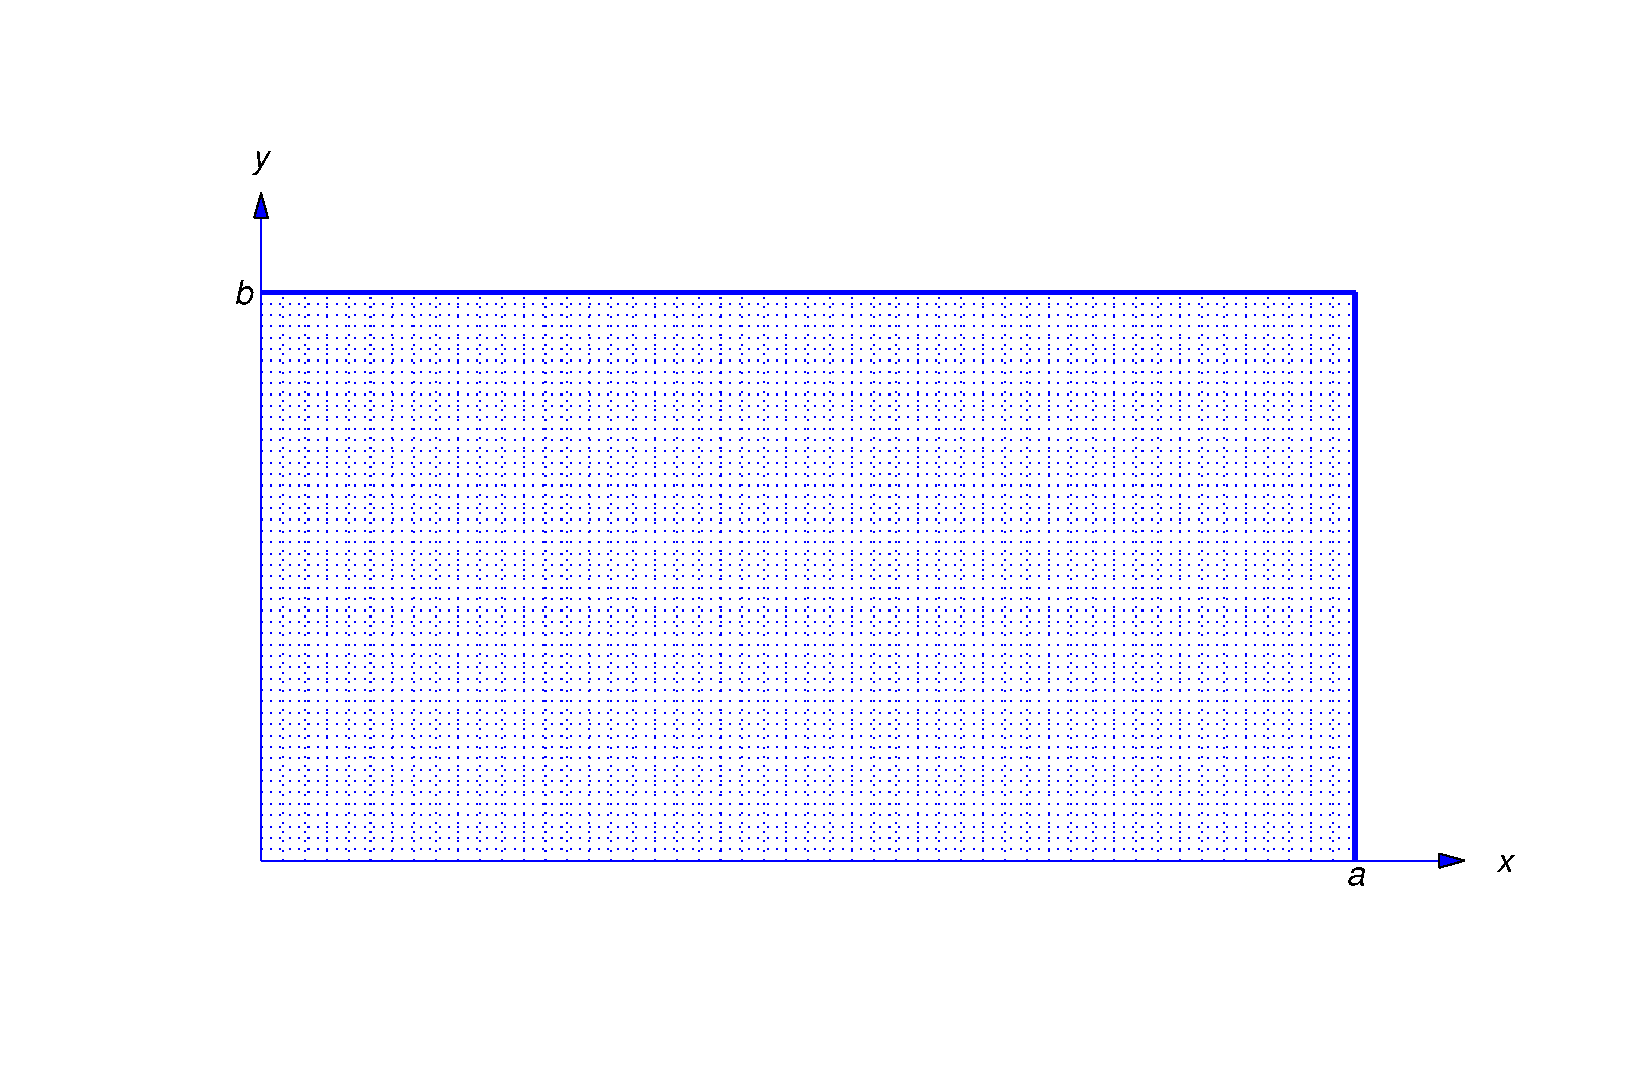
\includegraphics[bb=-78 148 689 643,width=5.67in,height=3.66in,keepaspectratio]{fig120301}
\caption{ A rectangular region and its boundary}
  \label{figure:12.3.1}
\end{figure}

The possible boundary conditions for this region can be written
as
$$
\begin{array}{lcllll}
(1-\alpha)u(x,0)&+&\alpha u_y(x,0)&=&f_0(x),  &0\le x\le
a,\\[2\jot]
(1-\beta) u(x,b)&+&\beta u_y(x,b)&=&f_1(x), &0\le x\le a,\\[2\jot]
(1-\gamma) u(0,y)&+&\gamma u_x(0,y)&=&g_0(y), &0\le y\le b,\\[2\jot]
(1-\delta) u(a,y)&+&\delta u_x(a,y)&=&g_1(y), &0\le y\le b,
\end{array}
$$
where $\alpha$, $\beta$, $\gamma$, and $\delta$  can each be either
$0$ or $1$;   thus, there are 16 possibilities.
Let
BVP$(\alpha,\beta,\gamma,\delta)(f_0,f_1,g_0,g_1)$
denote the problem of finding a solution of \eqref{eq:12.3.2} that
satisfies these conditions.
This is a Dirichlet problem if
$$
\alpha=\beta=\gamma=\delta=0
$$
(Figure~\ref{figure:12.3.2}),
or a Neumann problem if
$$
\alpha=\beta=\gamma=\delta=1
$$
(Figure~\ref{figure:12.3.3}).
The other 14 problems  are mixed.

\begin{figure}[htbp]
\color{blue}
  \begin{minipage}[b]{0.5\linewidth}
    \centering
   \scalebox{.5}{
  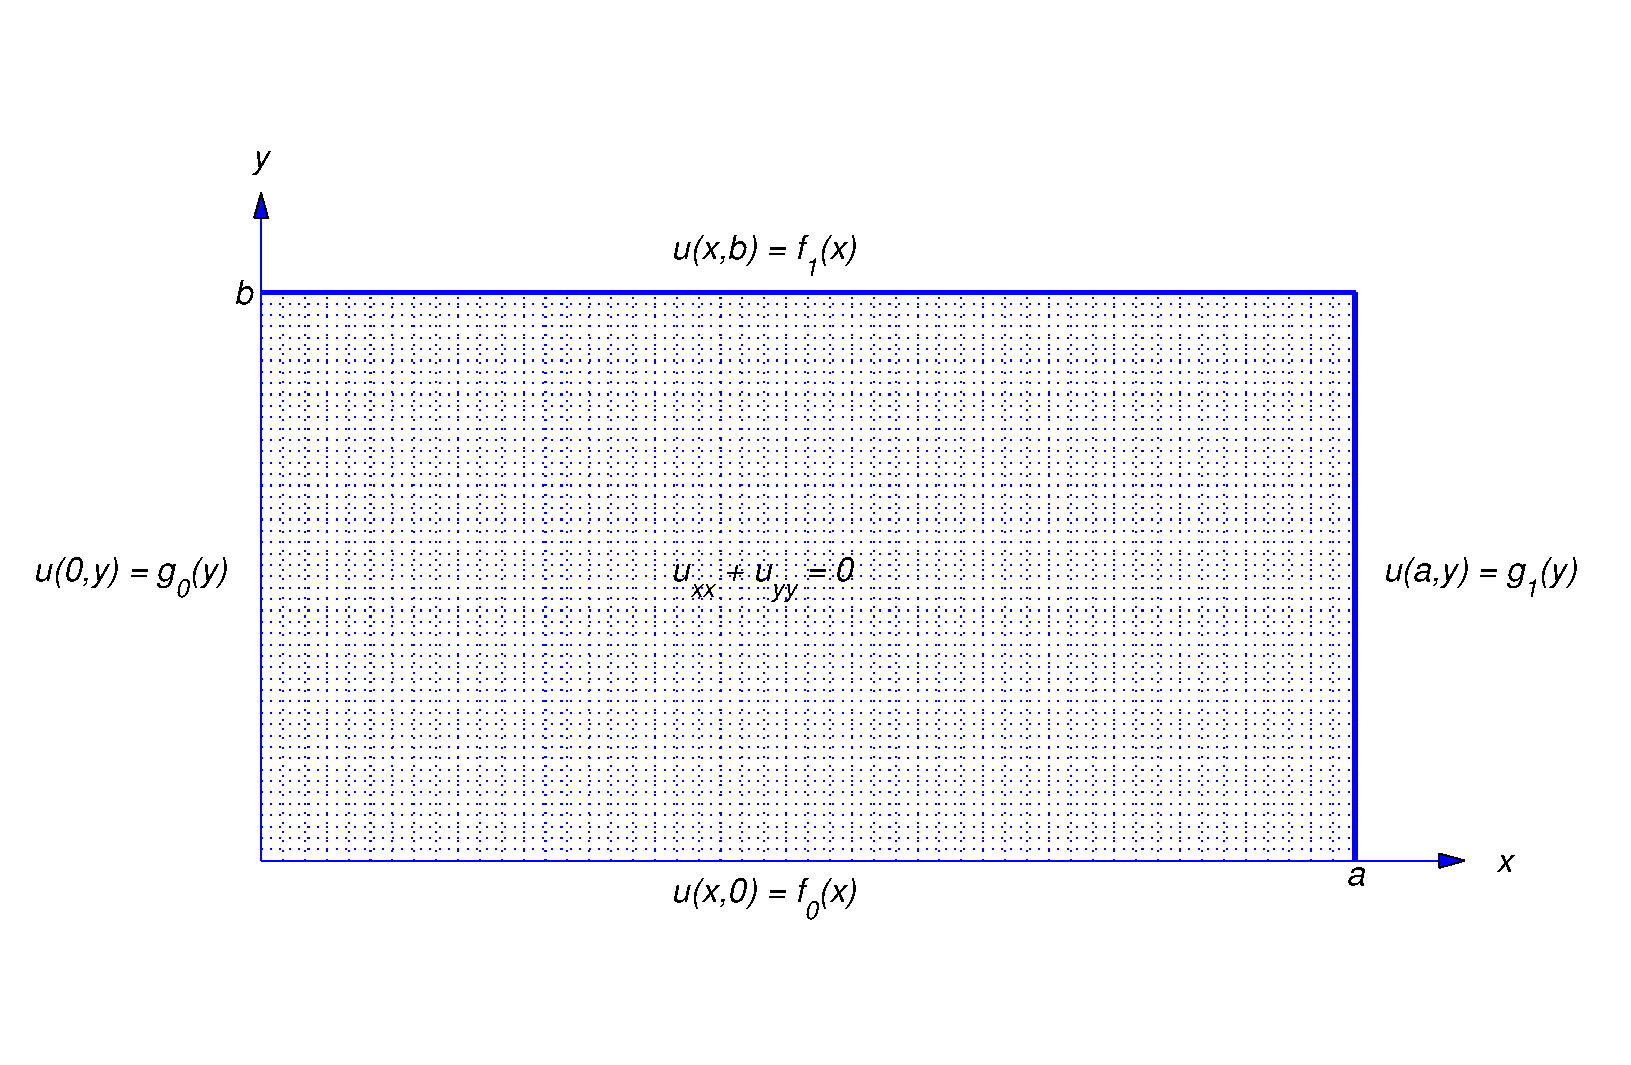
\includegraphics[bb=-78 148 689 643,width=5.67in,height=3.66in,keepaspectratio]{fig120302}}
\caption{ A Dirichlet problem}
  \label{figure:12.3.2}
\end{minipage}
  \begin{minipage}[b]{0.5\linewidth}
    \centering
   \scalebox{.5}{
  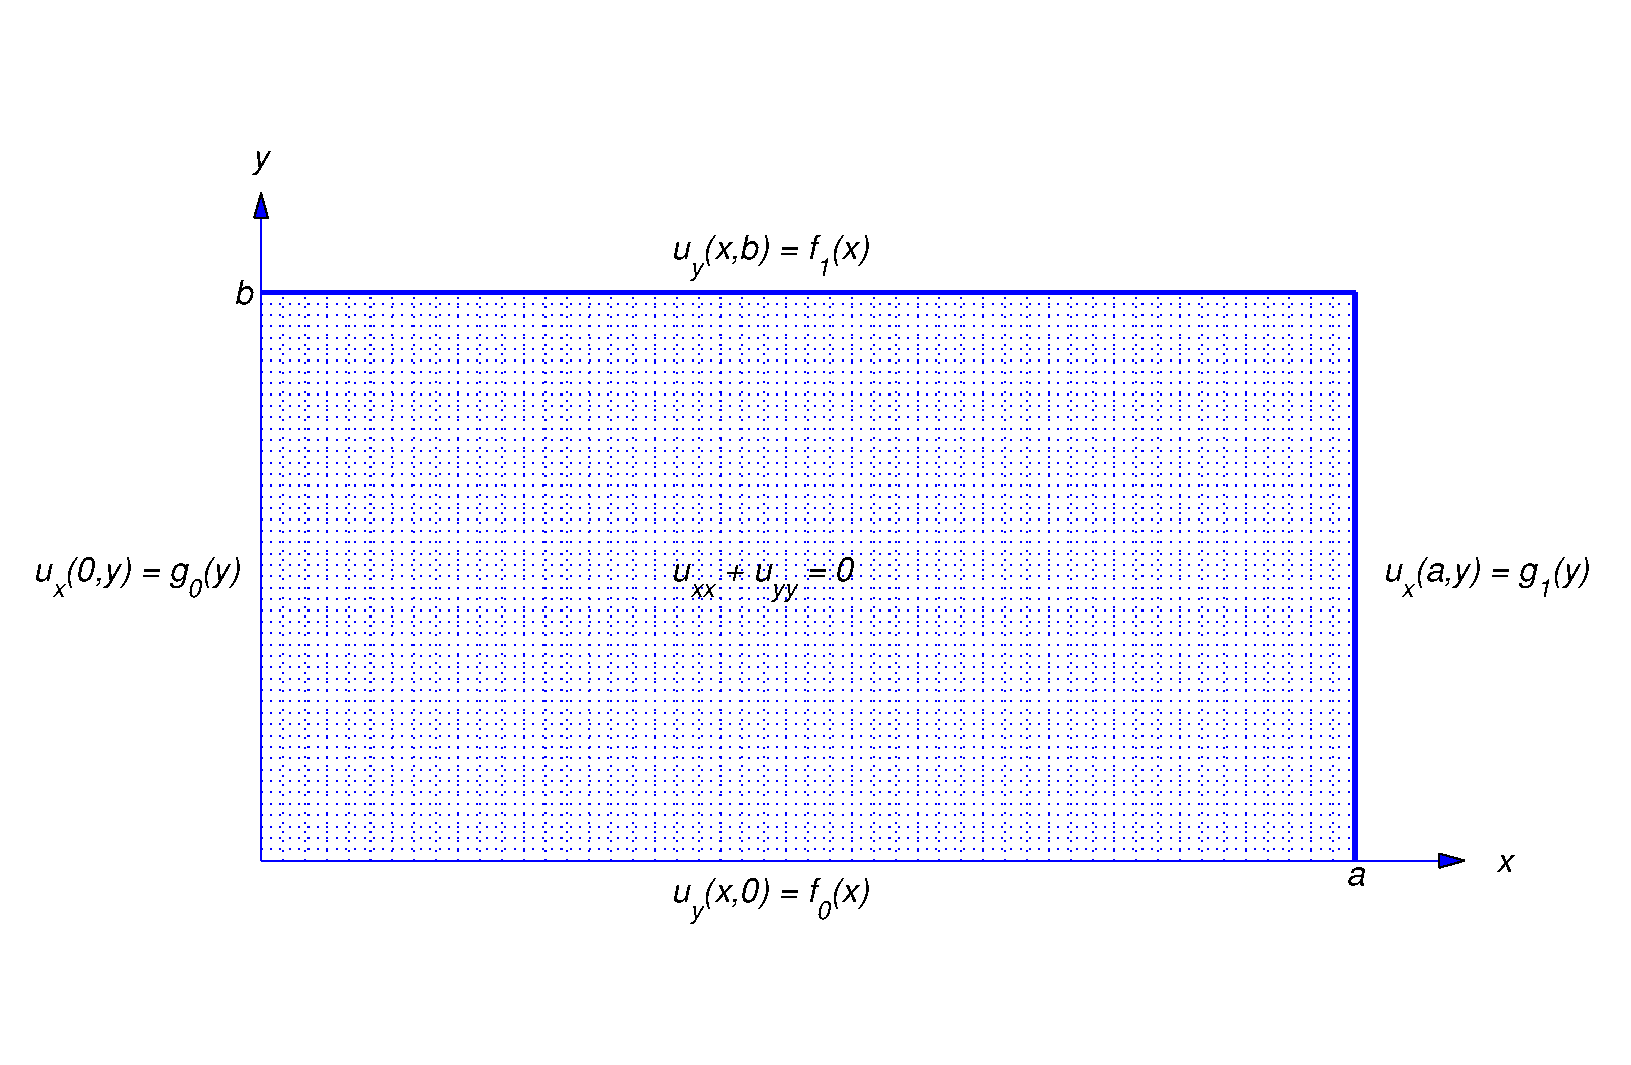
\includegraphics[bb=-78 148 689 643,width=5.67in,height=3.66in,keepaspectratio]{fig120303}}
\caption{ A Neumann problem}
  \label{figure:12.3.3}
\end{minipage}
\end{figure}

For given $(\alpha,\beta,\gamma,\delta)$, the sum of
solutions of
$$
\mbox{BVP}(\alpha,\beta,\gamma,\delta)(f_0,0,0,0),\quad
\mbox{BVP}(\alpha,\beta,\gamma,\delta)(0,f_1,0,0),
$$
$$
\mbox{BVP}(\alpha,\beta,\gamma,\delta)(0,0,g_0,0),
\mbox{\quad and \quad}
\mbox{BVP}(\alpha,\beta,\gamma,\delta)(0,0,0,g_1)
$$
is a solution of
$$
\mbox{BVP}(\alpha,\beta,\gamma,\delta)(f_0,f_1,g_0,g_1).
$$
 Therefore we  concentrate
on problems where only one of the functions $f_0$,
$f_1$,
$g_0$, $g_2$ isn't  identically zero. There are 64 (count them!)
 problems of this form. Each has homogeneous
boundary conditions on three sides of the rectangle, and a
nonhomogeneous boundary condition on the fourth. We  use
separation of variables to find infinitely many functions
that satisfy
Laplace's equation and the three homogeneous boundary
conditions in the open rectangle.
 We then use
these solutions as  building blocks to construct a formal solution of
Laplace's equation that also  satisfies the  nonhomogeneous
boundary condition.
Since it's not feasible to consider
all 64 cases, we'll restrict our attention in the text to
just four.  Others are discussed in the exercises.

If $v(x,y)=X(x)Y(y)$ then $$ v_{xx}+v_{yy}=X''Y+XY''=0 $$ for all
$(x,y)$ if and only if $$ {X''\over X}=-{Y''\over Y}=k $$ for all
$(x,y)$, where $k$ is a separation constant. This equation is
equivalent to
\begin{equation} \label{eq:12.3.3}
X''-kX=0,\quad  Y''+kY=0.
\end{equation}
From here,
the strategy  depends upon the
boundary conditions. We  illustrate this by examples.

\begin{example}\label{example:12.3.1} \rm
Define the formal solution of
\begin{equation} \label{eq:12.3.4}
\begin{array}{c}
u_{xx}+u_{yy}=0,\quad 0<x<a,\quad  0<y<b,\\
u(x,0)=f(x),\quad u(x,b)=0,\quad 0\le x\le a,\\
u(0,y)=0,\quad u(a,y)=0,\quad 0\le y\le b
\end{array}
\end{equation}
(Figure~\ref{figure:12.3.4}).
\end{example}

\begin{figure}[tbp]
  \centering\color{blue}
  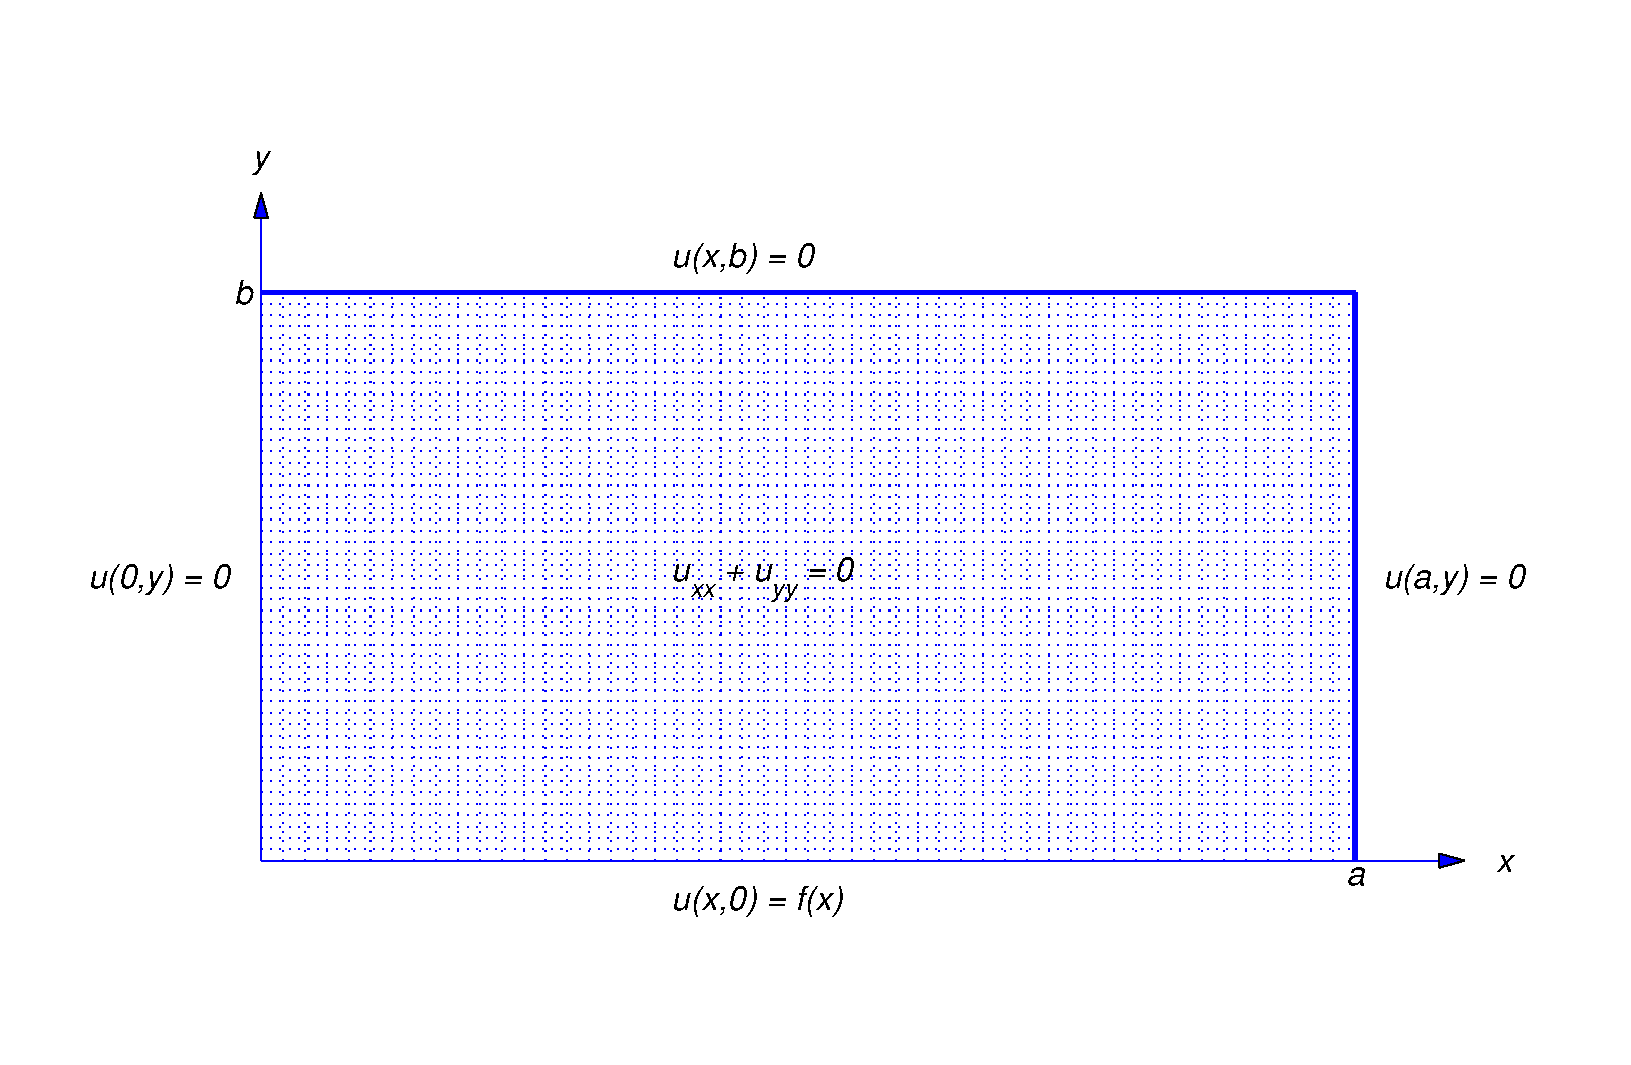
\includegraphics[bb=-78 148 689 643,width=5.67in,height=3.66in,keepaspectratio]{fig120304}
\caption{ The boundary value problem \eqref{eq:12.3.4}}
  \label{figure:12.3.4}
\end{figure}

\solution
The boundary conditions in \eqref{eq:12.3.4} require
 products $v(x,y)=X(x)Y(y)$ such that
$X(0)=X(a)=Y(b)=0$; hence, we let $k=-\lambda$ in \eqref{eq:12.3.3}.
Thus, $X$ and $Y$ must satisfy
\begin{equation} \label{eq:12.3.5}
X''+\lambda X=0,\quad X(0)=0,\quad X(a)=0
\end{equation}
and
\begin{equation} \label{eq:12.3.6}
Y''-\lambda Y=0,\quad Y(b)=0.
\end{equation}
 From Theorem~\ref{thmtype:11.1.2}, the eigenvalues of \eqref{eq:12.3.5}
are $\lambda_n=n^2\pi^2/a^2$, with
associated eigenfunctions
$$
X_n=\sin{n\pi x\over a}, \quad n=1,2,3,\dots.
$$
Substituting $\lambda=n^2\pi^2/a^2$  into
\eqref{eq:12.3.6} yields
$$
Y''-(n^2\pi^2/a^2)Y=0,\quad Y(b)=0,
$$
so we could take
\begin{equation} \label{eq:12.3.7}
Y_n=\sinh{n\pi(b-y)\over a};
\end{equation}
however, because of the nonhomogeneous Dirichlet  condition at $y=0$,
it's better to require that
$Y_n(0)=1$, which can be achieved by  dividing the right side
of
\eqref{eq:12.3.7} by its value at $y=0$;   thus, we take
$$
Y_n={\sinh n\pi(b-y)/a\over\sinh n\pi b/a}.
$$
Then
$$
v_n(x,y)=X_n(x)Y_n(y)={\sinh n\pi(b-y)/a\over\sinh n\pi b/a}\sin{n\pi
x\over a},
$$
so $v_n(x,0)=\sin n\pi x/a$ and
 $v_n$ satisfies \eqref{eq:12.3.4} with $f(x)=\sin n\pi x/a$. More
generally,
 if $\alpha_1$, \dots, $\alpha_m$ are arbitrary constants
then
$$
u_m(x,y)=\sum_{n=1}^m\alpha_n
{\sinh n\pi(b-y)/a\over\sinh n\pi b/a}
\sin{n\pi x\over a}
$$
satisfies \eqref{eq:12.3.4} with
$$
f(x)=\sum_{n=1}^m\alpha_n\sin{n\pi x\over L}.
$$
Therefore, if $f$ is an arbitrary piecewise smooth function on
$[0,a]$,  we define the formal solution of \eqref{eq:12.3.4} to be
\begin{equation} \label{eq:12.3.8}
u(x,y)=\sum_{n=1}^\infty \alpha_n
{\sinh n\pi(b-y)/a\over\sinh n\pi b/a}
\sin{n\pi x\over a},
\end{equation}
where
$$
S(x)=\sum_{n=1}^\infty \alpha_n\sin{n\pi x\over a}
$$
is the Fourier sine series of $f$ on $[0,a]$; that is,
$$
\alpha_n={2\over a}\int_0^af(x)\sin{n\pi x\over a}\,dx,\quad
n=1,2,3,\dots.
\eqno{\bbox}
$$

If $y<b$ then
\begin{equation} \label{eq:12.3.9}
{\sinh n\pi(b-y)/a\over\sinh n\pi b/a}\approx e^{-n\pi y/a}
\end{equation}
for large $n$,
so the series in \eqref{eq:12.3.8} converges if $0< y < b$;
 moreover, since also
$$
{\cosh n\pi(b-y)/a\over\sinh n\pi b/a}\approx e^{-n\pi y/a}
$$
for large $n$, Theorem~\ref{thmtype:12.1.2}
 applied twice with
 $z=x$ and  twice with  $z=t$, shows that   $u_{xx}$  and $u_{yy}$
can be obtained by differentiating $u$ term by term if $0<y<b$.
 (Exercise~\ref{exer:12.3.37}). Therefore $u$
satisfies Laplace's equation in the interior of the rectangle
in Figure~\ref{figure:12.3.4}.
Moreover, the series in \eqref{eq:12.3.8}
also converges on the boundary of the rectangle, and satisfies
the three homogeneous boundary conditions
conditions in \eqref{eq:12.3.4}.
 Therefore, since $u(x,0)=S(x)$ for $0\le x\le
L$, $u$ is an actual solution of \eqref{eq:12.3.5} if and only if
$S(x)=f(x)$ for $0\le x\le a$.
From Theorem~\ref{thmtype:11.3.2}, this is true if $f$
is continuous and piecewise smooth on $[0,L]$,
and $f(0)=f(L)=0$.

\begin{example}\label{example:12.3.2} \rm
Solve \eqref{eq:12.3.4} with $f(x)=x(x^2-3ax+2a^2)$.
\end{example}

\solution  From Example~\ref{example:11.3.6},
$$
S(x)={12a^3\over\pi^3}\sum_{n=1}^\infty{1\over n^3}\sin{n\pi
x\over a}.
$$
Therefore
\begin{equation} \label{eq:12.3.10}
u(x,y)={12a^3\over\pi^3}\sum_{n=1}^\infty{\sinh n\pi(b-y)/a\over
n^3\sinh n\pi b/a}
\sin{n\pi x\over a}.
\end{equation}

To compute approximate values of $u(x,y)$, we must use partial sums of
the form
$$
u_m(x,y)={12a^3\over\pi^3}\sum_{n=1}^m{\sinh n\pi(b-y)/a\over
n^3\sinh n\pi b/a}
\sin{n\pi x\over a}.
$$
Because of \eqref{eq:12.3.9}, small values of $m$
provide  sufficient accuracy for most applications if $0<y<b$.
Moreover, the
$n^3$ in the denominator in \eqref{eq:12.3.10} ensures that this is also
true for $y=0$.
 For graphing purposes, we chose $a=2$, $b=1$,
and $m=10$.
Figure~\ref{figure:12.3.5}  shows the surface
$$
u=u(x,y),\quad 0\le x\le 2,\quad 0\le y\le1,
$$
while Figure~\ref{figure:12.3.6}  shows the curves
$$
u=u(x,0.1k),\quad 0\le x\le2,\quad k=0,1,\dots,10.
$$

\begin{figure}[H]
\color{blue}
  \begin{minipage}[b]{0.5\linewidth}
    \centering
   \scalebox{.65}{
  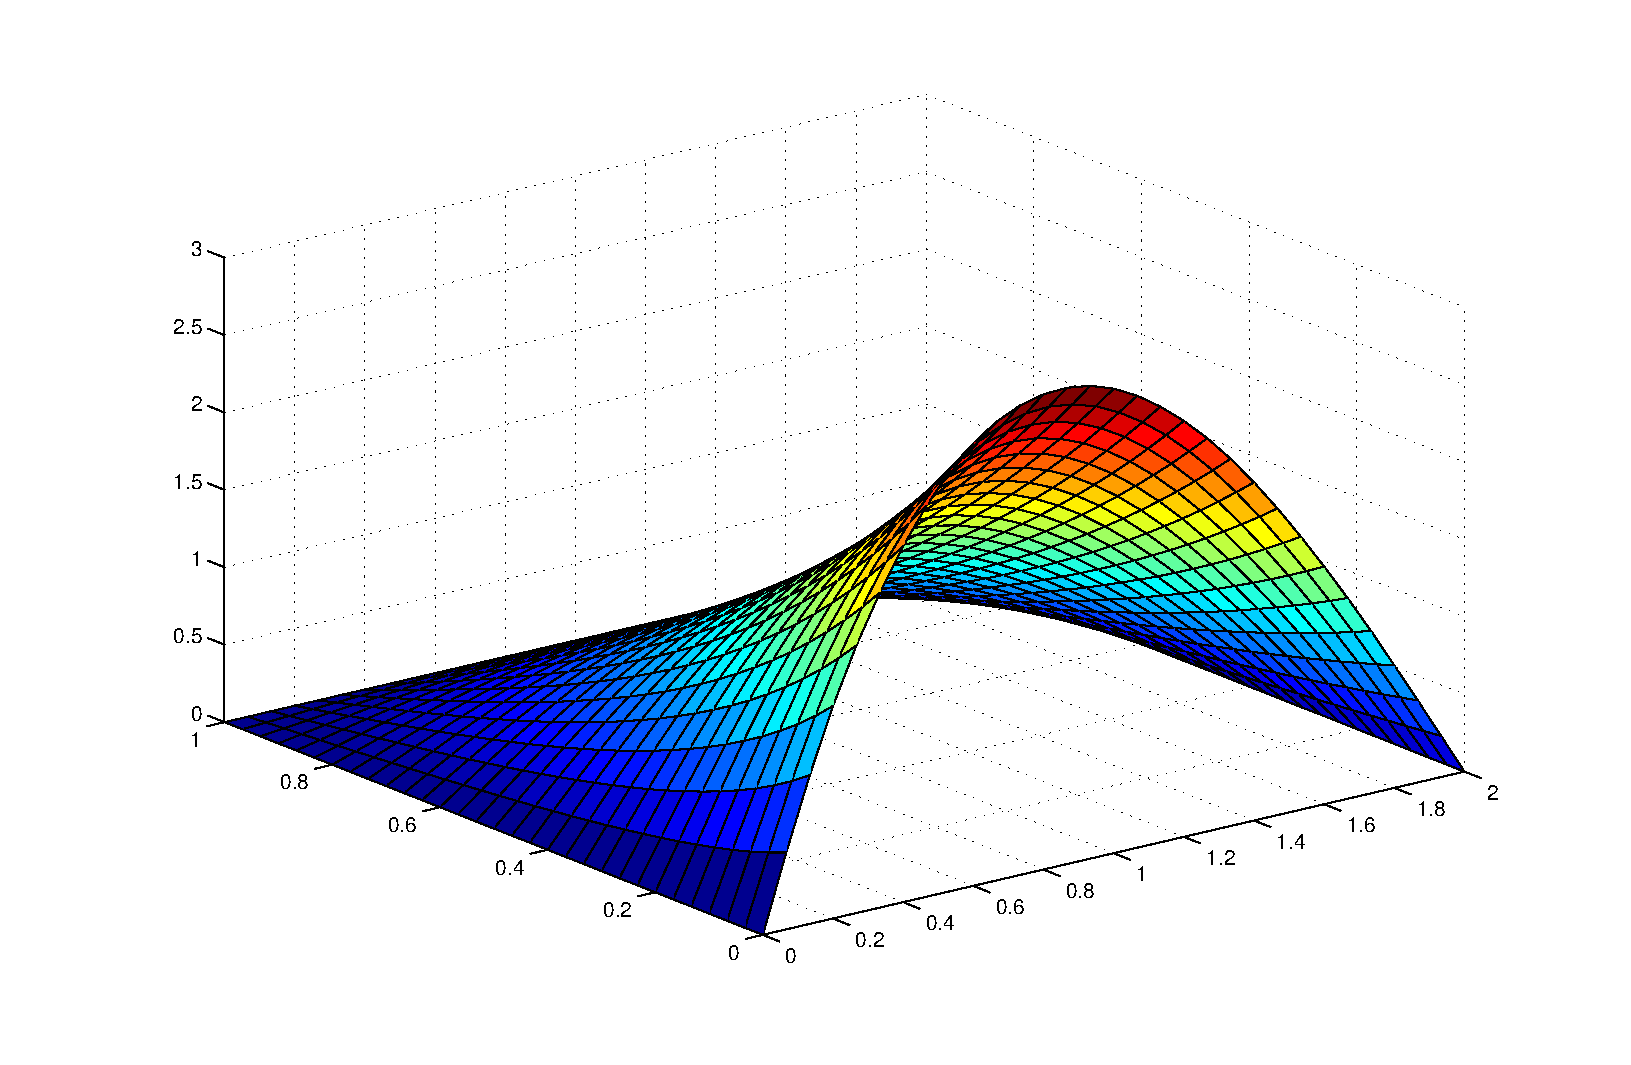
\includegraphics[bb=-78 148 689 643,width=5.67in,height=3.66in,keepaspectratio]{fig120305}}
  \caption{}
  \label{figure:12.3.5}
\end{minipage}
  \begin{minipage}[b]{0.5\linewidth}
    \centering
   \scalebox{.65}{
  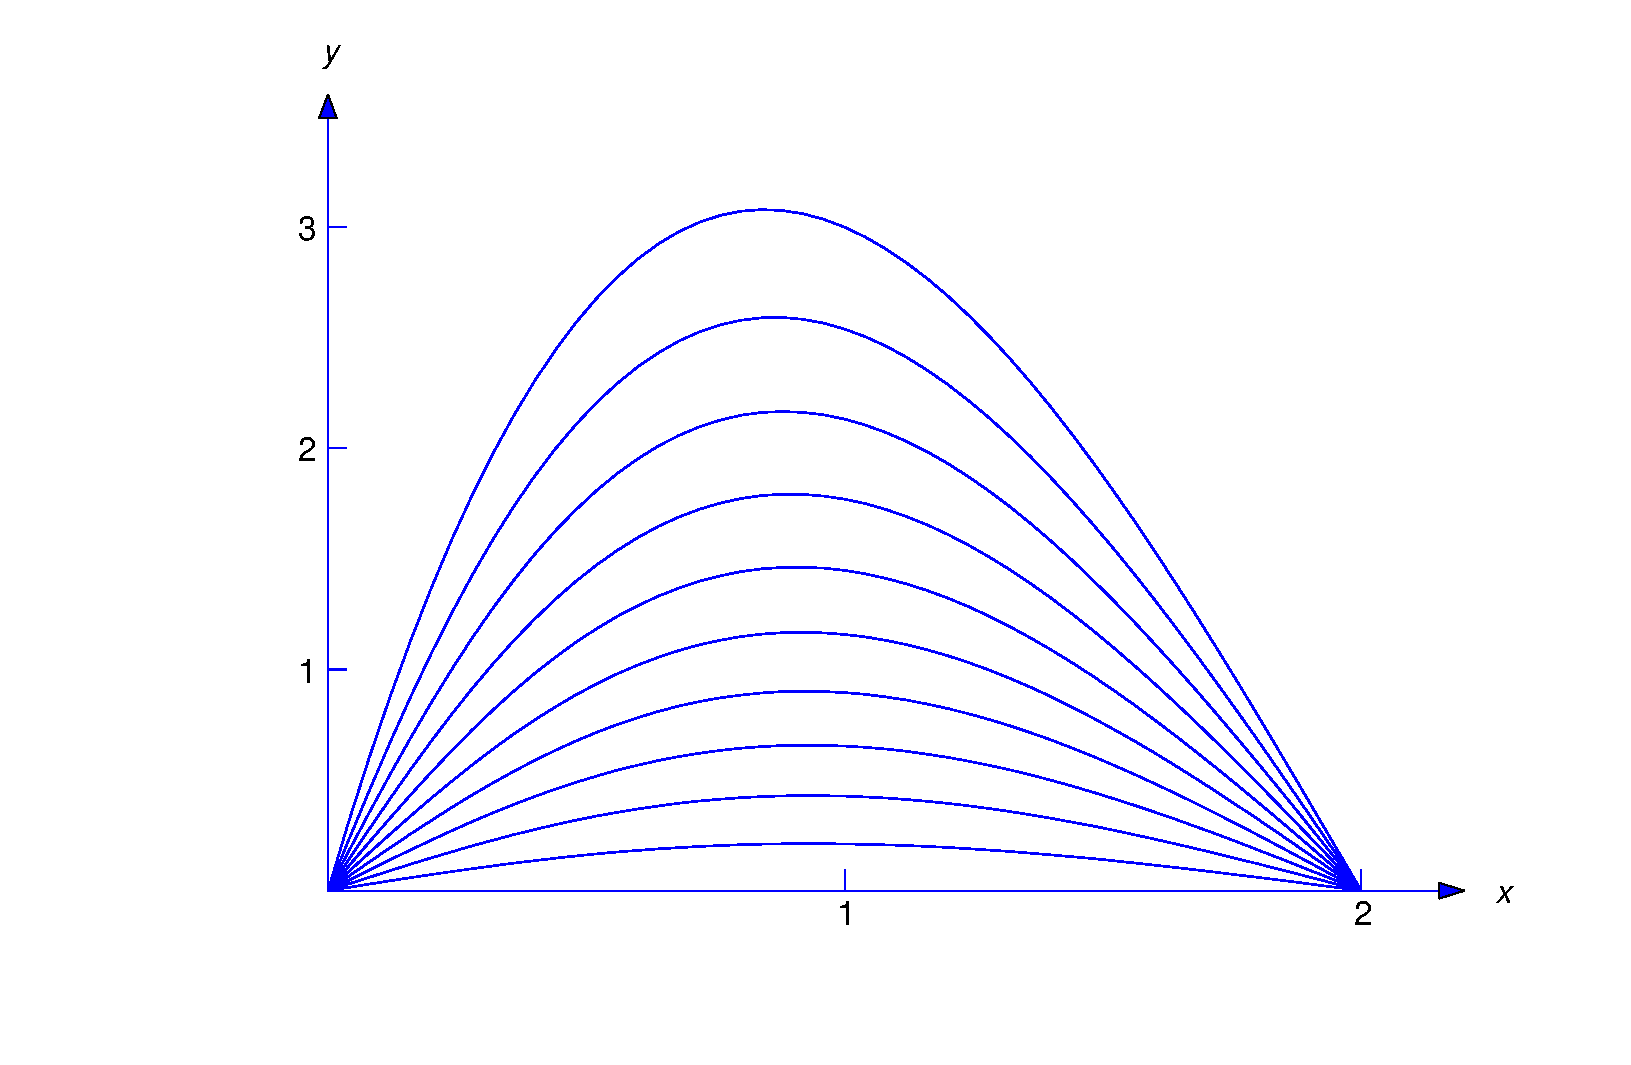
\includegraphics[bb=-78 148 689 643,width=5.67in,height=3.66in,keepaspectratio]{fig120306}}
  \caption{}
  \label{figure:12.3.6}
\end{minipage}
\end{figure}

\begin{example}\label{example:12.3.3}    \rm
Define the formal solution of
\begin{equation} \label{eq:12.3.11}
\begin{array}{c}
u_{xx}+u_{yy}=0,\quad 0<x<a,\quad  0<y<b,\\
u(x,0)=0,\quad u_y(x,b)=f(x),\quad 0\le x\le a,\\
u_x(0,y)=0,\quad u_x(a,y)=0,\quad 0\le y\le b
\end{array}
\end{equation}
(Figure~\ref{figure:12.3.7}).
\end{example}

\begin{figure}[H]
  \centering\color{blue}
  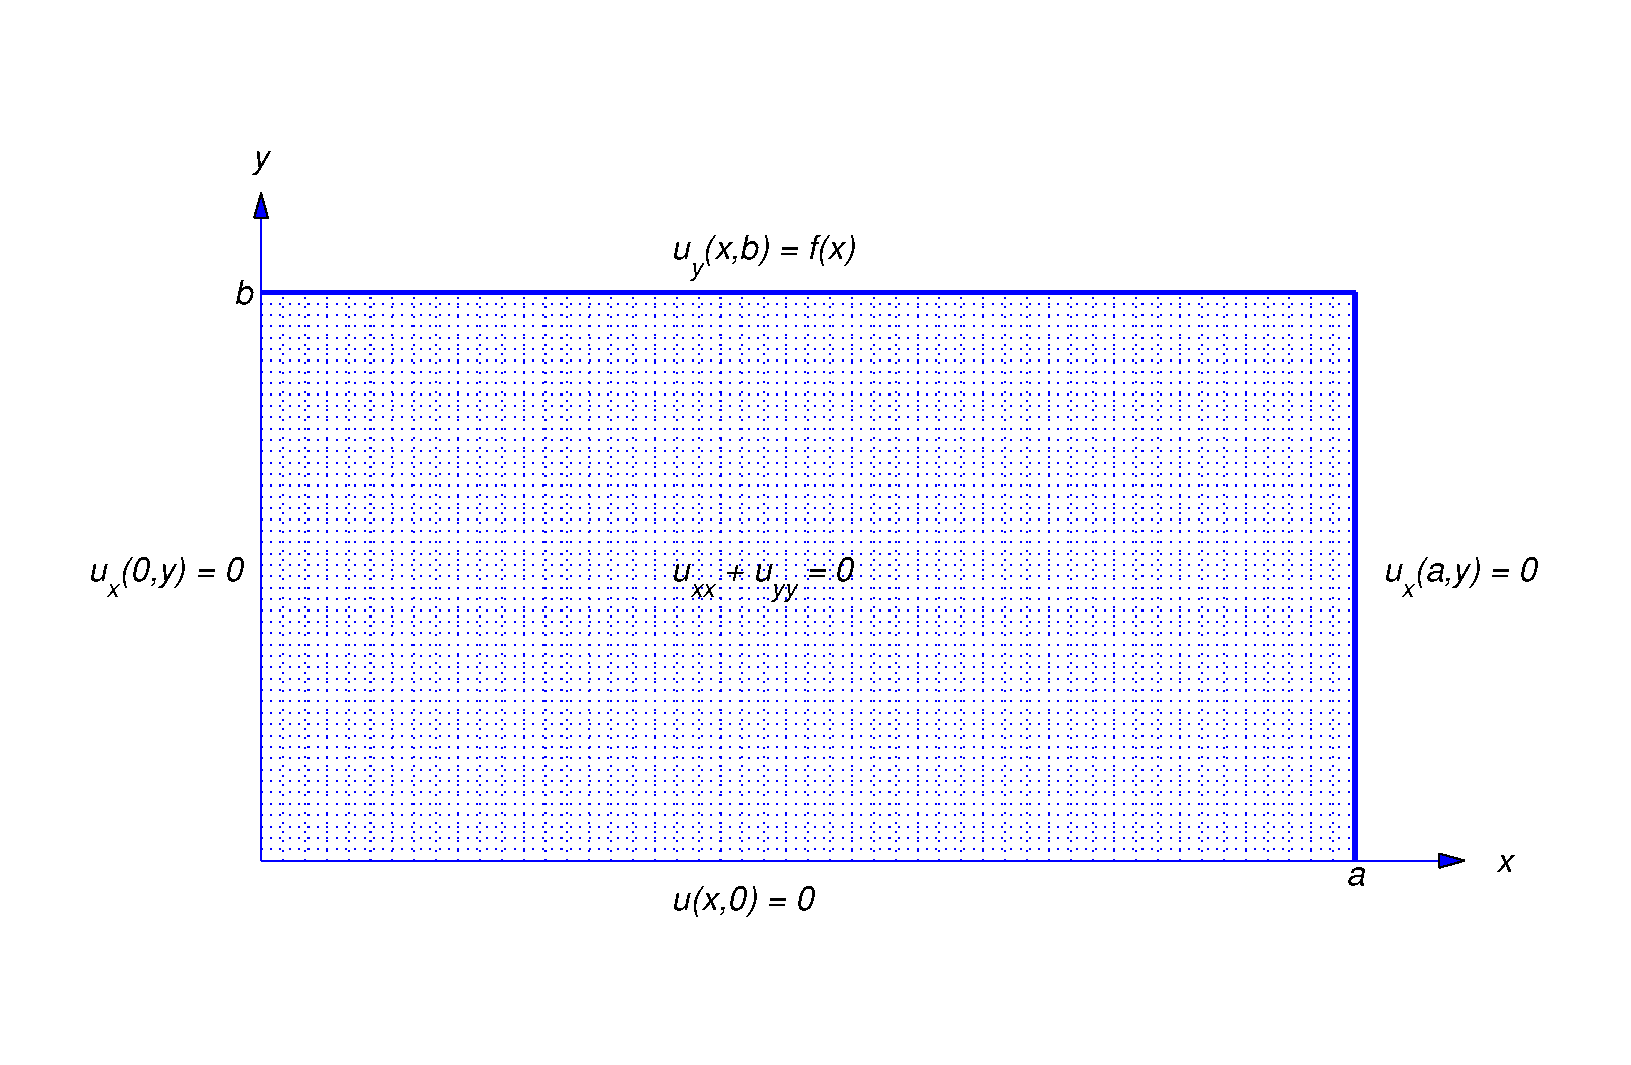
\includegraphics[bb=-78 148 689 643,width=5.67in,height=3.66in,keepaspectratio]{fig120307}
\caption{ The boundary value problem \eqref{eq:12.3.11}}
  \label{figure:12.3.7}
\end{figure}

\solution
The boundary conditions in \eqref{eq:12.3.11} require
 products $v(x,y)=X(x)Y(y)$ such that
$X'(0)=X'(a)=Y(0)=0$; hence, we let $k=-\lambda$ in
\eqref{eq:12.3.3}. Thus, $X$ and $Y$ must satisfy
\begin{equation} \label{eq:12.3.12}
X''+\lambda X=0,\quad X'(0)=0,\quad X'(a)=0
\end{equation}
and
\begin{equation} \label{eq:12.3.13}
Y''-\lambda Y=0,\quad Y(0)=0.
\end{equation}
 From Theorem~\ref{thmtype:11.1.3}, the eigenvalues of \eqref{eq:12.3.12}
are $\lambda=0$, with associated
eigenfunction $X_0=1$, and $\lambda_n=n^2\pi^2/a^2$, with
associated eigenfunctions
$$
X_n=\cos{n\pi x\over a}, \quad n=1,2,3,\dots.
$$
Since $Y_0=y$ satisfies \eqref{eq:12.3.13} with $\lambda=0$,
we take $v_0(x,y)=X_0(x)Y_0(y)= y$.
Substituting $\lambda=n^2\pi^2/a^2$  into
\eqref{eq:12.3.13} yields
$$
Y''-(n^2\pi^2/a^2)Y=0,\quad Y(0)=0,
$$
so we could take
\begin{equation} \label{eq:12.3.14}
Y_n=\sinh{n\pi y\over a}.
\end{equation}
However, because of the nonhomogeneous Neumann condition at $y=b$, it's
better to require that
$Y_n'(b)=1$, which can be achieved by  dividing the right side
of
\eqref{eq:12.3.14} by the value of its derivative  at $y=b$; thus,
$$
Y_n={a\sinh n\pi y/a\over n\pi\cosh n\pi b/a}.
$$
Then
$$
v_n(x,y)=X_n(x)Y_n(y)=
{a\sinh n\pi y/a\over n\pi\cosh n\pi b/a}\cos{n\pi x\over a},
$$
so
$$
{\partial v_n\over \partial y}(x,b)=\cos{n\pi x\over a}.
$$
Therefore
 $v_n$ satisfies \eqref{eq:12.3.11} with $f(x)=\cos n\pi x/a$. More
generally,
 if $\alpha_0$, \dots, $\alpha_m$ are arbitrary constants
then
$$
u_m(x,y)=\alpha_0y+{a\over\pi}\sum_{n=1}^m\alpha_n
{\sinh n\pi y/a\over n\cosh n\pi b/a}
\cos{n\pi x\over a}
$$
satisfies \eqref{eq:12.3.11} with
$$
f(x)=\alpha_0+\sum_{n=1}^m\alpha_n\cos{n\pi x\over L}.
$$
Therefore, if $f$ is an arbitrary piecewise smooth function on
$[0,a]$  we define the formal solution of \eqref{eq:12.3.11} to be
$$
u(x,y)=\alpha_0y+{a\over\pi}\sum_{n=1}^\infty \alpha_n
{\sinh n\pi y/a\over n\cosh n\pi b/a}
\cos{n\pi x\over a},
$$
where
$$
C(x)=\alpha_0+\sum_{n=1}^\infty \alpha_n\cos{n\pi x\over a}
$$
is the Fourier cosine series of $f$ on $[0,a]$; that is,
$$
\alpha_0={1\over a}\int_0^af(x)\,dx
\mbox{\quad and \quad}
\alpha_n={2\over a}\int_0^af(x)\cos{n\pi x\over a}\,dx,\quad
n=1,2,3,\dots.
$$

\begin{example}\label{example:12.3.4}\rm
Solve \eqref{eq:12.3.11} with $f(x)=x$.
\end{example}

\solution From Example~\ref{example:11.3.1},
$$
C(x)=\dst{a\over2}-{4a\over\pi^2}\sum_{n=1}^\infty{1\over(2n-1)^2}
\cos{(2n-1)\pi x\over a}.
$$
Therefore
\begin{equation} \label{eq:12.3.15}
u(x,y)=\dst{ay\over2}-{4a^2\over\pi^3}\sum_{n=1}^\infty
{\sinh(2n-1)\pi y/a\over(2n-1)^3\cosh(2n-1)\pi b/a}
\cos{(2n-1)\pi x\over a}.
\end{equation}
 For graphing purposes, we chose $a=2$, $b=1$,
and retained the terms through $n=10$ in  \eqref{eq:12.3.15}.
Figure~\ref{figure:12.3.8}  shows the surface
$$
u=u(x,y),\quad 0\le x\le 2,\quad 0\le y\le1,
$$
while Figure~\ref{figure:12.3.9}  shows the curves
$$
u=u(x,.1k),\quad 0\le x\le2,\quad k=0,1,\dots,10.
$$

\begin{figure}[H]
\color{blue}
  \begin{minipage}[b]{0.5\linewidth}
    \centering
   \scalebox{.65}{
  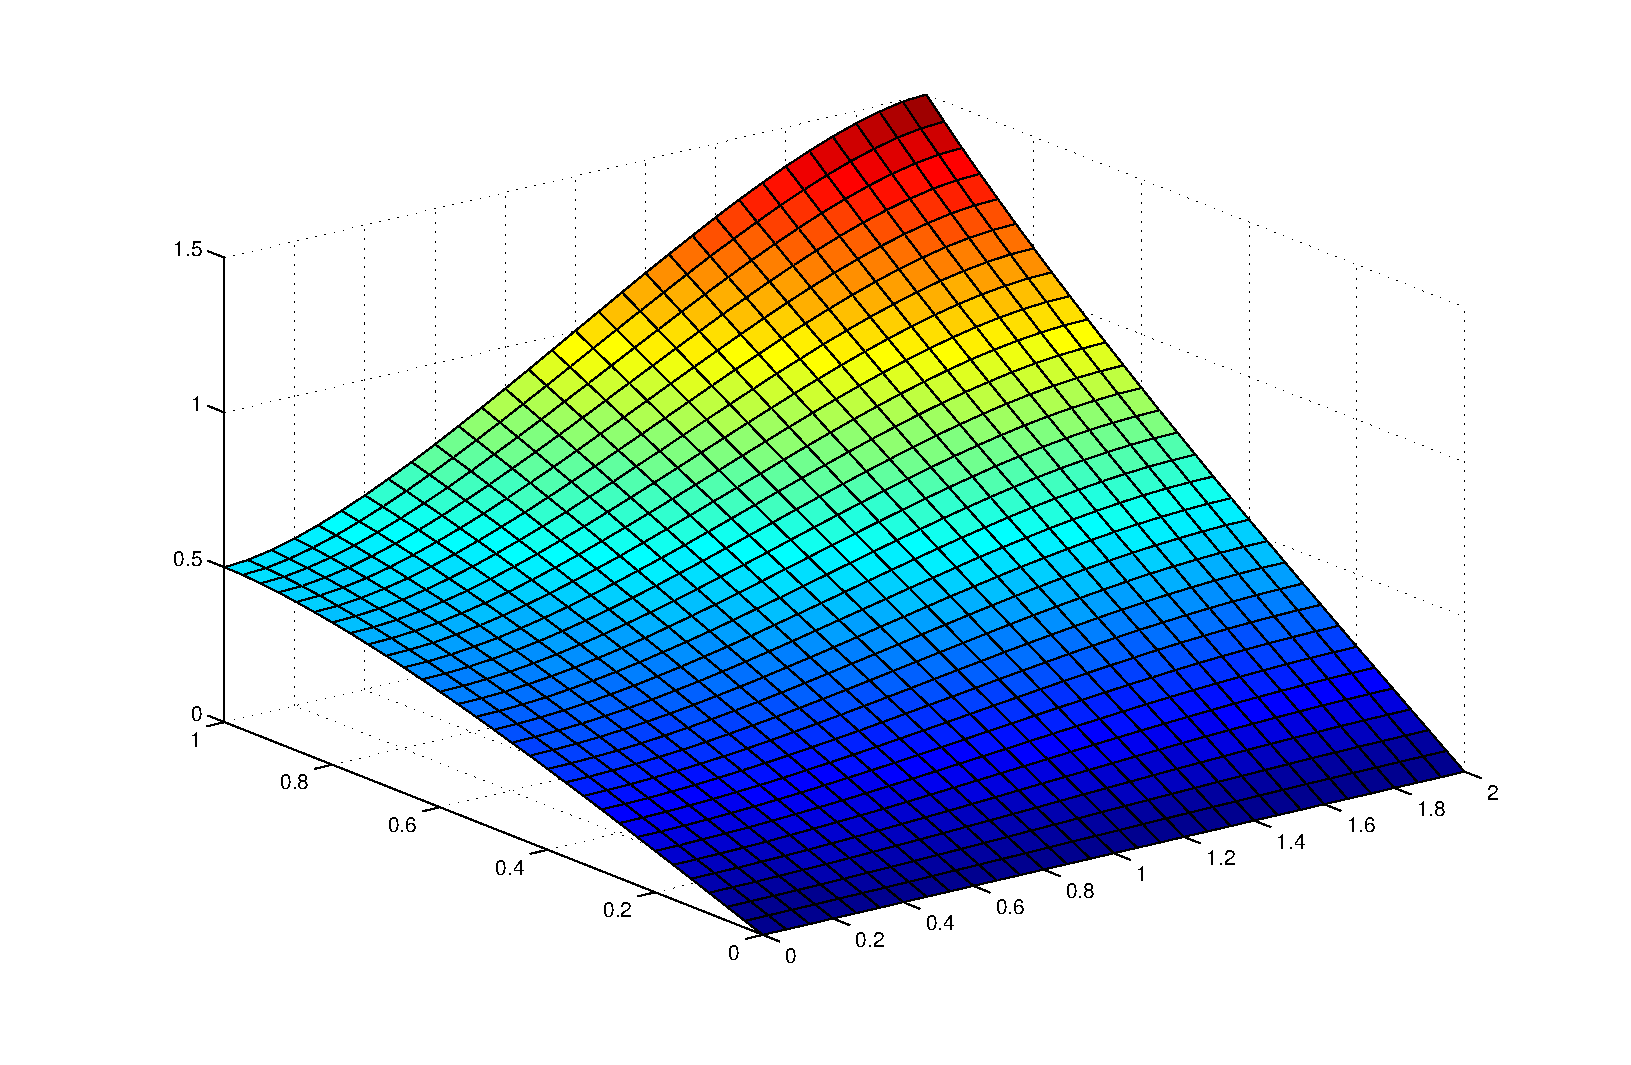
\includegraphics[bb=-78 148 689 643,width=5.67in,height=3.66in,keepaspectratio]{fig120308}}
  \caption{}
  \label{figure:12.3.8}
\end{minipage}
  \begin{minipage}[b]{0.5\linewidth}
    \centering
   \scalebox{.65}{
  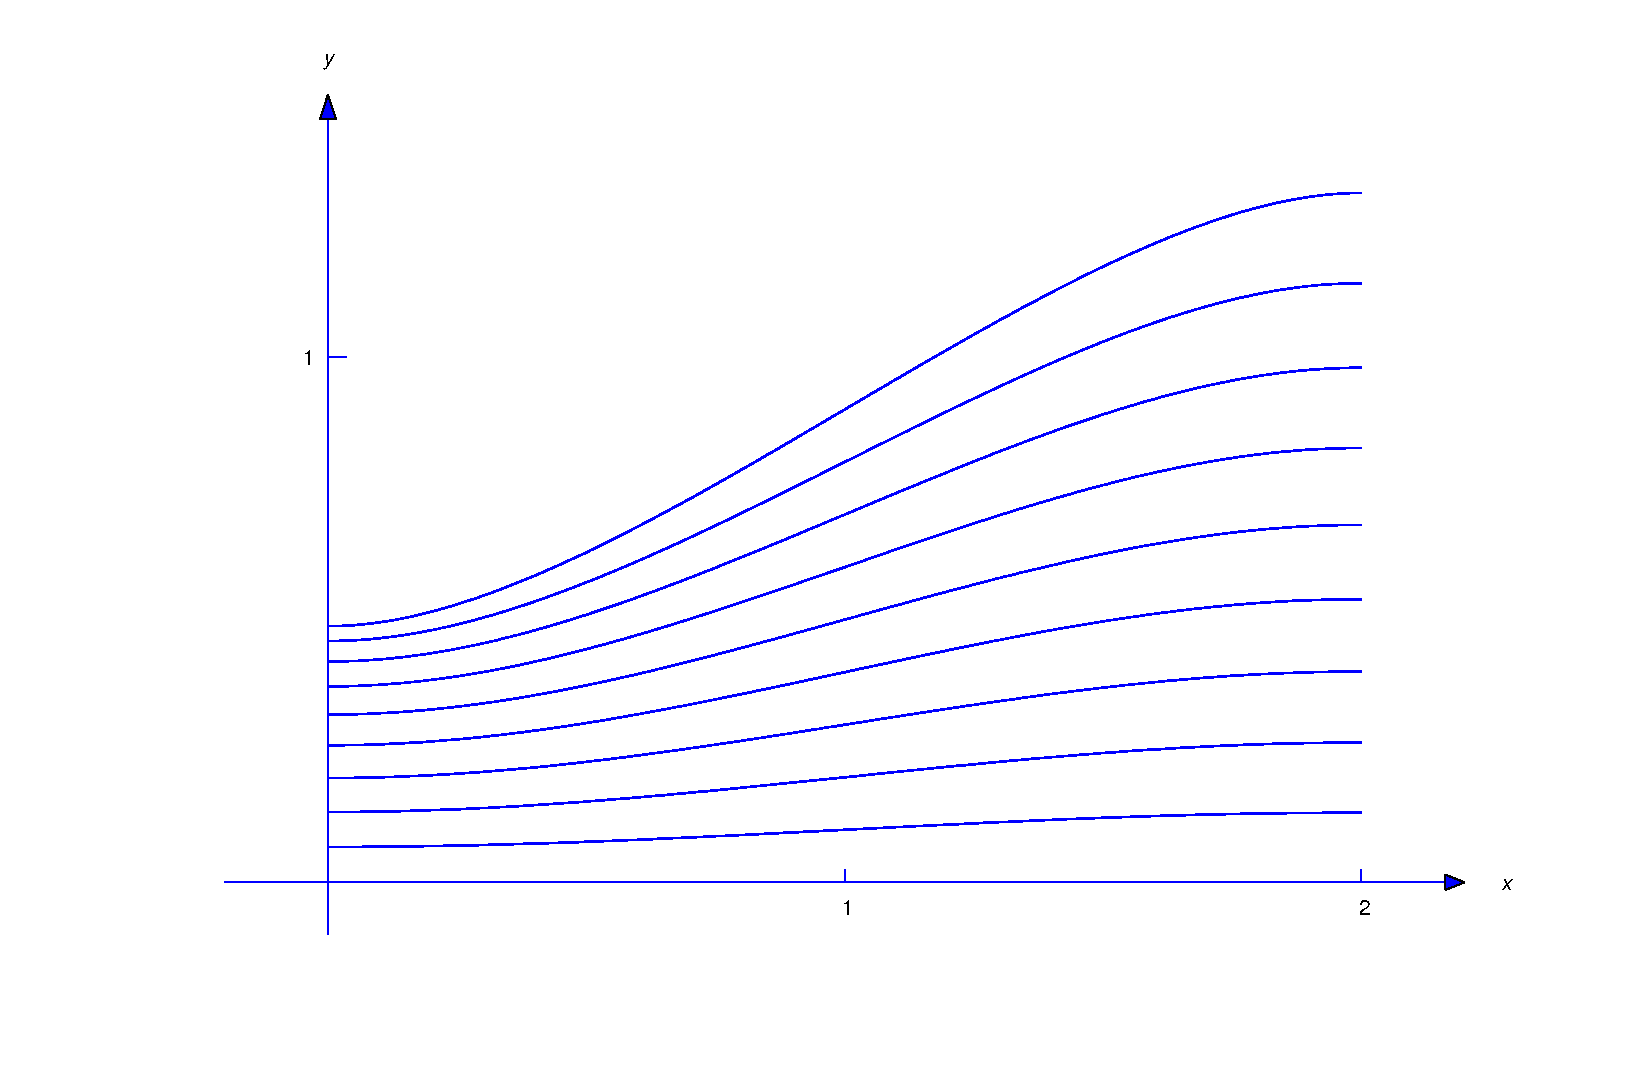
\includegraphics[bb=-78 148 689 643,width=5.67in,height=3.66in,keepaspectratio]{fig120309}}
  \caption{}
  \label{figure:12.3.9}
\end{minipage}
\end{figure}

\begin{example}\label{example:12.3.5} \rm
Define the formal solution of
\begin{equation} \label{eq:12.3.16}
\begin{array}{c}
u_{xx}+u_{yy}=0,\quad 0<x<a,\quad  0<y<b,\\
u(x,0)=0,\quad u_y(x,b)=0,\quad 0\le x\le a,\\
u(0,y)=g(y),\quad u_x(a,y)=0,\quad 0\le y\le b
\end{array}
\end{equation}
(Figure~\ref{figure:12.3.10}).
\end{example}

\begin{figure}[tbp]
  \centering\color{blue}
  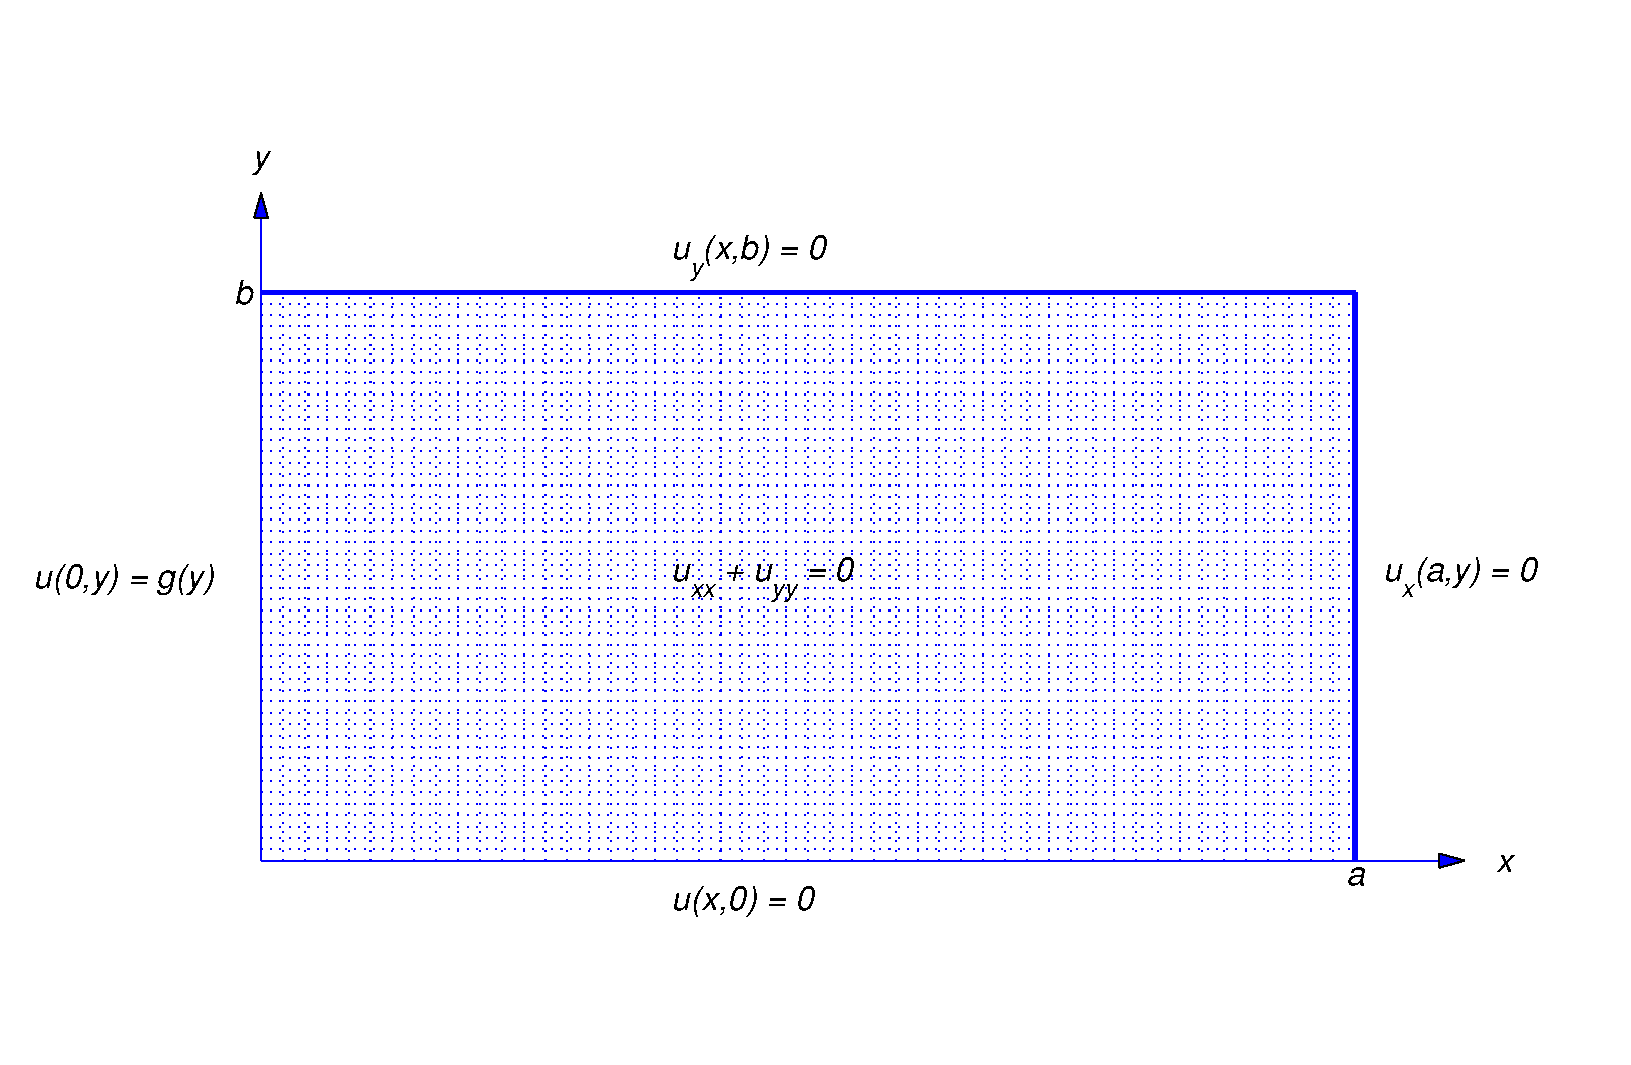
\includegraphics[bb=-78 148 689 643,width=5.67in,height=3.66in,keepaspectratio]{fig120310}
\caption{ The boundary value problem \eqref{eq:12.3.16}}
  \label{figure:12.3.10}
\end{figure}

\solution
The boundary conditions in \eqref{eq:12.3.16} require
 products $v(x,y)=X(x)Y(y)$ such that
$Y(0)=Y'(b)=X'(a)=0$; hence, we let $k=\lambda$ in
\eqref{eq:12.3.3}. Thus, $X$ and $Y$ must satisfy
\begin{equation} \label{eq:12.3.17}
X''-\lambda X=0,\quad \quad X'(a)=0
\end{equation}
and
\begin{equation} \label{eq:12.3.18}
Y''+\lambda Y=0,\quad Y(0)=0,\quad Y'(b)=0.
\end{equation}
 From Theorem~\ref{thmtype:11.1.4}, the eigenvalues of \eqref{eq:12.3.18}
are $\lambda_n=(2n-1)^2\pi^2/4b^2$, with
associated eigenfunctions
$$
Y_n=\sin{(2n-1)\pi y\over2b}, \quad n=1,2,3,\dots.
$$
Substituting $\lambda=(2n-1)^2\pi^2/4b^2$  into
\eqref{eq:12.3.17} yields
$$
X''-((2n-1)^2\pi^2/4b^2)X=0,\quad X'(a)=0,
$$
so we could take
\begin{equation} \label{eq:12.3.19}
X_n=\cosh{(2n-1)\pi(x-a)\over 2b}.
\end{equation}
However, because of the nonhomogeneous Dirichlet condition at $x=0$, it's
better to require that
$X_n(0)=1$, which can be achieved by  dividing the right side
of
\eqref{eq:12.3.19} by its  value  at $x=0$; thus,
$$
X_n=
{\cosh(2n-1)\pi(x-a)/2b\over\cosh(2n-1)\pi a/2b}.
$$
Then
$$
v_n(x,y)=X_n(x)Y_n(y)=
{\cosh(2n-1)\pi(x-a)/2b\over\cosh(2n-1)\pi a/2b}\sin{(2n-1)\pi
y\over2b},
$$
so
$$
v_n(0,y)=\sin{(2n-1)\pi y\over2b}.
$$
Therefore
 $v_n$ satisfies \eqref{eq:12.3.16} with $g(y)=\sin(2n-1)\pi y/2b$. More
generally,
 if $\alpha_1$, \dots, $\alpha_m$ are arbitrary constants
then
$$
u_m(x,y)=\sum_{n=1}^m \alpha_n
{\cosh(2n-1)\pi(x-a)/2b\over\cosh(2n-1)\pi a/2b}\sin{(2n-1)\pi y\over 2b}
$$
satisfies \eqref{eq:12.3.16} with
$$
g(y)=\sum_{n=1}^m \alpha_n\sin{(2n-1)\pi
y\over2b}.
$$
Thus, if $g$ is an arbitrary piecewise smooth function on
$[0,b]$,  we define the formal solution of \eqref{eq:12.3.16} to be
$$
u(x,y)=\sum_{n=1}^\infty \alpha_n
{\cosh(2n-1)\pi(x-a)/2b\over\cosh(2n-1)\pi a/2b}\sin{(2n-1)\pi y\over 2b},
$$
where
$$
S_M(x)=\sum_{n=1}^\infty \alpha_n\sin{(2n-1)\pi
y\over2b}
$$
 is the mixed Fourier sine series of $g$ on $[0,b]$;
that is,
$$
\alpha_n={2\over b}\int_0^bg(y)\sin{(2n-1)\pi y\over2b}\,dy.
$$

\begin{example}\label{example:12.3.6} \rm
Solve \eqref{eq:12.3.16} with $g(y)=y(2y^2-9by+12b^2)$.
\end{example}

\solution  From Example~\ref{example:11.3.8},
$$
S_M(y)
=\dst{96b^3\over\pi^3}\sum_{n=1}^\infty
{1\over(2n-1)^3}\left[3+(-1)^n{4\over(2n-1)\pi}\right]\sin{(2n-1)\pi
y\over2b}.
$$
Therefore
$$
u(x,y)
=\dst{96b^3\over\pi^3}\sum_{n=1}^\infty
{\cosh(2n-1)\pi(x-a)/2b\over(2n-1)^3\cosh(2n-1)\pi a/2b}
\left[3+(-1)^n{4\over(2n-1)\pi}\right]\sin{(2n-1)\pi
y\over2b}.
$$

\begin{example}\label{example:12.3.7} \rm
Define the formal solution of
\begin{equation} \label{eq:12.3.20}
\begin{array}{c}
u_{xx}+u_{yy}=0,\quad 0<x<a,\quad  0<y<b,\\
u_y(x,0)=0,\quad u(x,b)=0,\quad 0\le x\le a,\\
u_x(0,y)=0,\quad u_x(a,y)=g(y),\quad 0\le y\le b
\end{array}
\end{equation}
(Figure~\ref{figure:12.3.11}).
\end{example}

\begin{figure}[tbp]
  \centering\color{blue}
  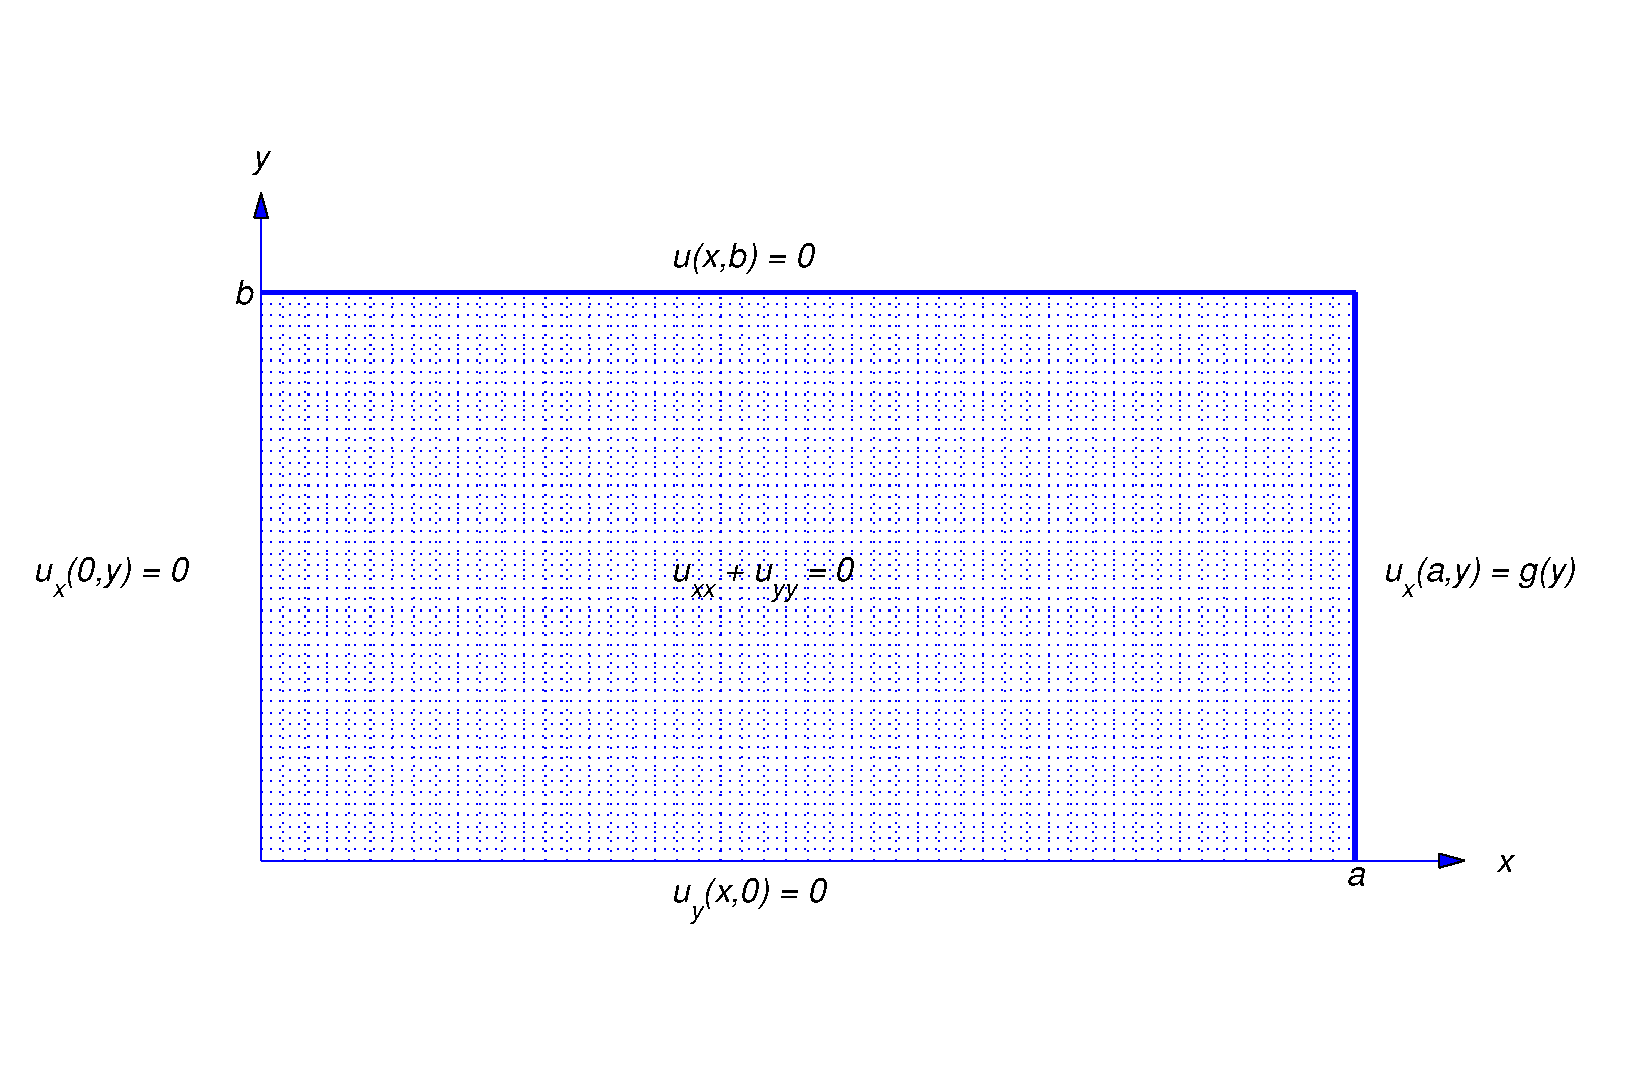
\includegraphics[bb=-78 148 689 643,width=5.67in,height=3.66in,keepaspectratio]{fig120311}
\caption{ The boundary value problem \eqref{eq:12.3.20}}
  \label{figure:12.3.11}
\end{figure}

\solution
The boundary conditions in \eqref{eq:12.3.20} require
 products $v(x,y)=X(x)Y(y)$ such that
$Y'(0)=Y(b)=X'(0)=0$; hence, we let $k=\lambda$ in
\eqref{eq:12.3.3}. Thus, $X$ and $Y$ must satisfy
\begin{equation} \label{eq:12.3.21}
X''-\lambda X=0,\quad \quad X'(0)=0
\end{equation}
and
\begin{equation} \label{eq:12.3.22}
Y''+\lambda Y=0,\quad Y'(0)=0,\quad Y(b)=0.
\end{equation}
 From Theorem~\ref{thmtype:11.1.4}, the eigenvalues of \eqref{eq:12.3.22}
are $\lambda_n=(2n-1)^2\pi^2/4b^2$, with
associated eigenfunctions
$$
Y_n=\cos{(2n-1)\pi y\over2b}, \quad n=1,2,3,\dots.
$$
Substituting $\lambda=(2n-1)^2\pi^2/4b^2$  into
\eqref{eq:12.3.21} yields
$$
X''-((2n-1)^2\pi^2/4b^2)X=0,\quad X'(0)=0,
$$
so we could take
\begin{equation} \label{eq:12.3.23}
X_n=\cosh{(2n-1)\pi x\over 2b}.
\end{equation}
However, because of the nonhomogeneous Neumann condition at $x=a$, it's
better to require that
$X_n'(a)=1$, which can be achieved by  dividing the right side
of
\eqref{eq:12.3.23} by the   value of its derivative  at $x=a$; thus,
$$
X_n=
{2b\cosh(2n-1)\pi x/2b\over(2n-1)\pi\sinh(2n-1)\pi a/2b}.
$$
Then
$$
v_n(x,y)=X_n(x)Y_n(y)=
{2b\cosh(2n-1)\pi x/2b\over(2n-1)\pi\sinh(2n-1)\pi a/2b}\cos{(2n-1)\pi
y\over2b},
$$
so
$$
{\partial v_n\over\partial x}(a,y)=\cos{(2n-1)\pi y\over2b}.
$$
Therefore
 $v_n$ satisfies \eqref{eq:12.3.20} with $g(y)=\cos(2n-1)\pi y/2b$. More
generally,
 if $\alpha_1$, \dots, $\alpha_m$ are arbitrary constants
then
$$
u_m(x,y)={2b\over\pi}\sum_{n=1}^m \alpha_n
{\cosh(2n-1)\pi x/2b\over(2n-1)\sinh(2n-1)\pi a/2b}\cos{(2n-1)\pi y\over 2b}
$$
satisfies \eqref{eq:12.3.20} with
$$
g(y)=\sum_{n=1}^\infty \alpha_n\cos{(2n-1)\pi
y\over2b}.
$$
Therefore, if $g$ is an arbitrary piecewise smooth function on
$[0,b]$,  we define the formal solution of \eqref{eq:12.3.20} to be
$$
u(x,y)={2b\over\pi}\sum_{n=1}^\infty \alpha_n
{\cosh(2n-1)\pi x/2b\over(2n-1)\sinh(2n-1)\pi a/2b}\cos{(2n-1)\pi y\over 2b},
$$
where
$$
C_M(y)=\sum_{n=1}^\infty \alpha_n\cos{(2n-1)\pi
y\over2b}
$$
 is the mixed Fourier cosine series of $g$ on $[0,b]$;
that is,
$$
\alpha_n={2\over b}\int_0^bg(y)\cos{(2n-1)\pi y\over2b}\,dy.
$$

\begin{example}\label{example:12.3.8}    \rm
Solve \eqref{eq:12.3.20} with $g(y)=y-b$.
\end{example}

\solution  From Example~\ref{example:11.3.3},
$$
C_M(y)=-{8b\over\pi^2}\sum_{n=1}^\infty{1\over(2n-1)^2}
\cos{(2n-1)\pi y\over2b}.
$$
Therefore
$$
u(x,y)=-{16b^2\over\pi^3}\sum_{n=1}^\infty{
\cosh(2n-1)\pi x/2b\over(2n-1)^3\sinh(2n-1)\pi a/2b}
\cos{(2n-1)\pi y\over2b}.
\eqno{\bbox}
$$

\boxit{Laplace's Equation for a Semi-Infinite Strip}

\noindent
We now seek solutions of Laplace's equation on
the semi-infinite strip
$$
S:\{0<x<a,\quad y>0\}
$$
(Figure~\ref{figure:12.3.12})
that satisfy homogeneous boundary conditions at $x=0$ and $x=a$, and
a nonhomogeneous  Dirichlet or Neumann condition at $y=0$. An
example of such a problem is
\begin{equation} \label{eq:12.3.24}
\begin{array}{c}
u_{xx}+u_{yy}=0,\quad 0<x<a,\quad  y>0,\\
u(x,0)=f(x),\quad 0\le x\le a,\\
u(0,y)=0,\quad u(a,y)=0,\quad y>0,
\end{array}
\end{equation}

   \begin{figure}[tbp]
  \centering\color{blue}
  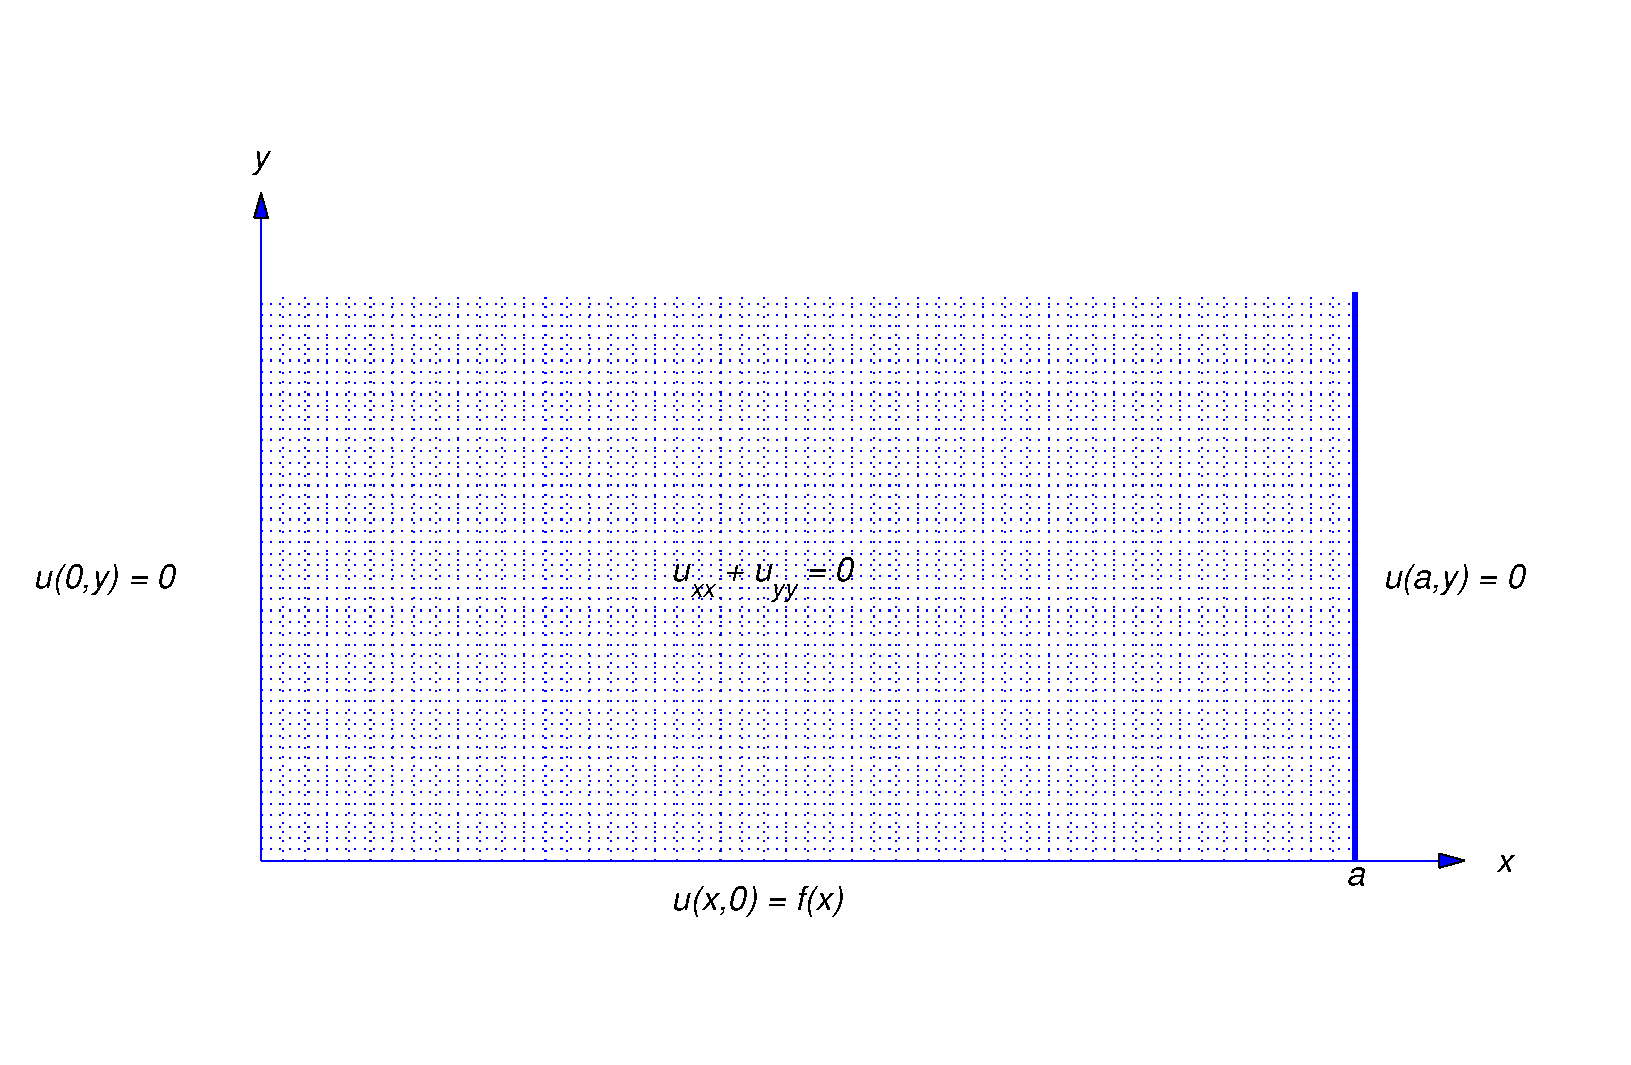
\includegraphics[bb=-78 148 689 643,width=5.67in,height=3.66in,keepaspectratio]{fig120312}
\caption{ A boundary value problem on a semi-infinite strip}
  \label{figure:12.3.12}
\end{figure}

The boundary conditions in this problem are not sufficient to
determine
$u$, for if $u_0=u_0(x,y)$ is a solution
and $K$ is a constant then
$$
u_1(x,y)=u_0(x,y)+K\sin{\pi x\over a}\sinh{\pi y\over a}.
$$
is also a solution. (Verify.) However, if we also require ---
on physical grounds --- that the solution remain bounded
for all $(x,y)$ in $S$
 then $K=0$ and this difficulty is eliminated.

\begin{example}\label{example:12.3.9} \rm
Define the bounded formal solution of
\eqref{eq:12.3.24}.
\end{example}

\solution Proceeding as in the solution of Example~\ref{example:12.3.1},
we find that the building block functions are of the form
$$
v_n(x,y)=Y_n(y)\sin{n\pi x\over a},
$$
where
$$
Y_n''-(n^2\pi^2/a^2)Y_n=0.
$$
Therefore
$$
Y_n=c_1e^{n\pi y/a}+c_2e^{-n\pi y/a}
$$
where $c_1$ and $c_2$ are constants.
Although the boundary conditions in \eqref{eq:12.3.24}  don't restrict
$c_1$, and $c_2$, we must set $c_1=0$ to ensure that $Y_n$ is bounded.
Letting $c_2=1$ yields
$$
v_n(x,y)=e^{-n\pi y/a}\sin{n\pi x\over a},
$$
and we define the bounded formal solution of \eqref{eq:12.3.24} to be
$$
u(x,y)=\sum_{n=1}^\infty b_ne^{-n\pi y/a}\sin{n\pi x\over a},
$$
where
$$
S(x)=\sum_{n=1}^\infty b_n\sin{n\pi x\over a}
$$
is the Fourier sine series of $f$ on $[0,a]$.
\bbox

See Exercises~\ref{exer:12.3.29}-\ref{exer:12.3.34}  for other boundary value
problems  on a semi-infinite strip.

\exercises
In Exercises~\ref{exer:12.3.1}-\ref{exer:12.3.16} apply the definition
developed in Example~1 to  solve the boundary
value problem. (Use Theorem~\ref{thmtype:11.3.5} where it
applies.)
 Where indicated by \Cex, graph the surface
$u=u(x,y)$, $0\le x\le a$, $0\le y\le b$.

\begin{exerciselist}

\item\label{exer:12.3.1}
$u_{xx}+u_{yy}=0,\quad 0<x<1,\quad  0<y<1,$\\
$u(x,0)=x(1-x),\quad u(x,1)=0,\quad 0\le x\le 1,$\\
$u(0,y)=0,\quad u(1,y)=0,\quad 0\le y\le 1$

\item\label{exer:12.3.2}
$u_{xx}+u_{yy}=0,\quad 0<x<2,\quad  0<y<3,$\\
$u(x,0)=x^2(2-x),\quad u(x,3)=0,\quad 0\le x\le 2,$\\
$u(0,y)=0,\quad u(2,y)=0,\quad 0\le y\le 3$

\item\label{exer:12.3.3}  \Cex
$u_{xx}+u_{yy}=0,\quad 0<x<2,\quad  0<y<2,$\\
$u(x,0)=
\left\{\begin{array}{cl}
x,& 0\le x\le 1,\\
2-x,&1\le x\le2,
\end{array}\right.
\quad u(x,2)=0,\quad 0\le x\le 2,$\\
$u(0,y)=0,\quad u(2,y)=0,\quad 0\le y\le 2$

\item\label{exer:12.3.4}
$u_{xx}+u_{yy}=0,\quad 0<x<\pi,\quad  0<y<1,$\\
$u(x,0)=x\sin x,\quad u(x,\pi)=0,\quad 0\le x\le \pi,$\\
$u(0,y)=0,\quad u(\pi,y)=0,\quad 0\le y\le 1$

\item\label{exer:12.3.5}
$u_{xx}+u_{yy}=0,\quad 0<x<3,\quad  0<y<2,$\\
$u(x,0)=0,\quad u_y(x,2)=x^2,\quad 0\le x\le 3,$\\
$u_x(0,y)=0,\quad u_x(3,y)=0,\quad 0\le y\le 2$

\item\label{exer:12.3.6}
$u_{xx}+u_{yy}=0,\quad 0<x<1,\quad  0<y<2,$\\
$u(x,0)=0,\quad u_y(x,2)=1-x,\quad 0\le x\le 1,$\\
$u_x(0,y)=0,\quad u_x(1,y)=0,\quad 0\le y\le 2$

\item\label{exer:12.3.7}
$u_{xx}+u_{yy}=0,\quad 0<x<2,\quad  0<y<2,$\\
$u(x,0)=0,\quad u_y(x,2)=x^2-4,\quad 0\le x\le 2,$\\
$u_x(0,y)=0,\quad u_x(2,y)=0,\quad 0\le y\le 2$

\item\label{exer:12.3.8}
$u_{xx}+u_{yy}=0,\quad 0<x<1,\quad  0<y<1,$\\
$u(x,0)=0,\quad u_y(x,1)=(x-1)^2,\quad 0\le x\le 1,$\\
$u_x(0,y)=0,\quad u_x(1,y)=0,\quad 0\le y\le 1$

\item\label{exer:12.3.9}   \Cex
$u_{xx}+u_{yy}=0,\quad 0<x<3,\quad  0<y<2,$\\
$u(x,0)=0,\quad u_y(x,2)=0,\quad 0\le x\le 3,$\\
$u(0,y)=y(4-y),\quad u_x(3,y)=0,\quad 0\le y\le 2$

\item\label{exer:12.3.10}
$u_{xx}+u_{yy}=0,\quad 0<x<2,\quad  0<y<1,$\\
$u(x,0)=0,\quad u_y(x,1)=0,\quad 0\le x\le 2,$\\
$u(0,y)=y^2(3-2y),\quad u_x(2,y)=0,\quad 0\le y\le 1$

\item\label{exer:12.3.11}
$u_{xx}+u_{yy}=0,\quad 0<x<2,\quad  0<y<2,$\\
$u(x,0)=0,\quad u_y(x,2)=0,\quad 0\le x\le 2,$\\
$u(0,y)=(y-2)^3+8,\quad u_x(2,y)=0,\quad 0\le y\le 2$

\item\label{exer:12.3.12}
$u_{xx}+u_{yy}=0,\quad 0<x<3,\quad  0<y<1,$\\
$u(x,0)=0,\quad u_y(x,1)=0,\quad 0\le x\le 3,$\\
$u(0,y)=y(2y^2-9y+12),\quad u_x(3,y)=0,\quad 0\le y\le 1$

\item\label{exer:12.3.13}  \Cex
$u_{xx}+u_{yy}=0,\quad 0<x<1,\quad  0<y<\pi,$\\
$u_y(x,0)=0,\quad u(x,\pi)=0,\quad 0\le x\le 1,$\\
$u_x(0,y)=0,\quad u_x(1,y)=\sin y,\quad 0\le y\le \pi$

\item\label{exer:12.3.14}
$u_{xx}+u_{yy}=0,\quad 0<x<2,\quad  0<y<3,$\\
$u_y(x,0)=0,\quad u(x,3)=0,\quad 0\le x\le 2,$\\
$u_x(0,y)=0,\quad u_x(2,y)=y(3-y),\quad 0\le y\le 3$

\item\label{exer:12.3.15}
$u_{xx}+u_{yy}=0,\quad 0<x<1,\quad  0<y<\pi,$\\
$u_y(x,0)=0,\quad u(x,\pi)=0,\quad 0\le x\le 1,$\\
$u_x(0,y)=0,\quad u_x(1,y)=\pi^2-y^2,\quad 0\le y\le \pi$

\item\label{exer:12.3.16}
$u_{xx}+u_{yy}=0,\quad 0<x<1,\quad  0<y<1,$\\
$u_y(x,0)=0,\quad u(x,1)=0,\quad 0\le x\le 1,$\\
$u_x(0,y)=0,\quad u_x(1,y)=1-y^3,\quad 0\le y\le 1$

\exercisetext{In
Exercises~\ref{exer:12.3.17}-\ref{exer:12.3.28} define the formal solution of
$$
u_{xx}+u_{yy}=0,\quad 0<x<a,\quad 0<y<b
$$
that satisfies the given boundary conditions for general $a$, $b$,
and $f$ or $g$.
Then solve the boundary value problem for the specified  $a$,
$b$, and  $f$ or $g$.
 (Use Theorem~\ref{thmtype:11.3.5} where it applies.)
Where indicated by \Cex, graph the surface
$u=u(x,y)$, $0\le x\le a$, $0\le y\le b$.}

\item\label{exer:12.3.17}  \Cex
$u(x,0)=0,\quad u(x,b)=f(x),\quad 0<x<a,\\
u(0,y)=0,\quad u(a,y)=0,\quad 0<y<b$  \\
$a=3$,\quad $b=2$,\quad $f(x)=x(3-x)$

\item\label{exer:12.3.18}
$u(x,0)=f(x),\quad u(x,b)=0,\quad 0<x<a,\\
u_x(0,y)=0,\quad u_x(a,y)=0,\quad 0<y<b$  \\
$a=2$,\quad $b=1$,\quad $f(x)=x^2(x-2)^2$

\item\label{exer:12.3.19}
$u(x,0)=f(x),\quad u(x,b)=0,\quad 0<x<a,\\
u_x(0,y)=0,\quad u(a,y)=0,\quad 0<y<b$  \\
$a=1$,\quad $b=2$,\quad $f(x)=3x^3-4x^2+1$

\item\label{exer:12.3.20}
$u(x,0)=f(x),\quad u(x,b)=0,\quad 0<x<a,\\
u(0,y)=0,\quad u_x(a,y)=0,\quad 0<y<b$  \\
$a=3$,\quad $b=2$,\quad $f(x)=x(6-x)$

\item\label{exer:12.3.21}
$u(x,0)=f(x),\quad u_y(x,b)=0,\quad 0<x<a,\\
u(0,y)=0,\quad u(a,y)=0,\quad 0<y<b$  \\
$a=\pi$,\quad $b=2$,\quad $f(x)=x(\pi^2-x^2)$

\item\label{exer:12.3.22}
$u_y(x,0)=0,\quad u(x,b)=f(x),\quad 0<x<a,\\
u_x(0,y)=0,\quad u_x(a,y)=0,\quad 0<y<b$  \\
$a=\pi$,\quad $b=1$,\quad $f(x)=x^2(x-\pi)^2$

\item\label{exer:12.3.23} \Cex
$u_y(x,0)=f(x),\quad u(x,b)=0,\quad 0<x<a,\\
u(0,y)=0,\quad u(a,y)=0,\quad 0<y<b$  \\
$a=\pi$,\quad  $b=1$,\quad
$f(x)=
\left\{\begin{array}{cl}
x,&0\le x\le{\pi\over2},\\\pi-x,&{\pi\over2}\le x\le \pi
\end{array}\right.$

\item\label{exer:12.3.24}
$u(x,0)=0,\quad u(x,b)=0,\quad 0<x<a,\\
u_x(0,y)=0,\quad u(a,y)=g(y),\quad 0<y<b$  \\
$a=1$,\quad $b=1$,\quad $g(y)=y(y^3-2y^2+1)$

\item\label{exer:12.3.25} \Cex
$u_y(x,0)=0,\quad u(x,b)=0,\quad 0<x<a,\\
u_x(0,y)=0,\quad u(a,y)=g(y),\quad 0<y<b$  \\
$a=2$,\quad $b=2$,\quad $g(y)=4-y^2$

\item\label{exer:12.3.26}
$u(x,0)=0,\quad u(x,b)=0,\quad 0<x<a,\\
u_x(0,y)=0,\quad u_x(a,y)=g(y),\quad 0<y<b$  \\
$a=1$, $b=4$,
$g(y)=
\left\{\begin{array}{cl}
y,&0\le y\le2,\\4-y,&2\le y\le 4
\end{array}\right.$

\item\label{exer:12.3.27}
$u(x,0)=0,\quad u_y(x,b)=0,\quad 0<x<a,\\
u_x(0,y)=g(y),\quad u_x(a,y)=0,\quad 0<y<b$  \\
$a=1$,\quad  $b=\pi$,\quad $g(y)=y^2(3\pi-2y)$

\item\label{exer:12.3.28}
$u_y(x,0)=0,\quad u_y(x,b)=0,\quad 0<x<a,\\
u_x(0,y)=g(y),\quad u(a,y)=0,\quad 0<y<b$  \\
$a=2$,\quad $b=\pi$,\quad $g(y)=y$

\exercisetext{In
Exercises~\ref{exer:12.3.29}-\ref{exer:12.3.34} define the bounded formal
solution of
$$
u_{xx}+u_{yy}=0,\quad 0<x<a,\quad y>0
$$
that satisfies the given boundary conditions for general $a$ and $f$.
Then solve the boundary value problem for the specified  $a$
and  $f$.}

\item\label{exer:12.3.29}
$u(x,0)=f(x),\quad 0<x<a$,\quad\\
$u_x(0,y)=0,\quad u_x(a,y)=0,\quad y>0$  \\
$a=\pi$   $f(x)=x^2(3\pi-2x)$

\item\label{exer:12.3.30}
$u(x,0)=f(x),\quad 0<x<a$,\\
$u_x(0,y)=0,\quad u(a,y)=0,\quad y>0$  \\
$a=3$,\quad $f(x)=9-x^2$

\item\label{exer:12.3.31}
$u(x,0)=f(x),\quad 0<x<a$,\quad\\
$u(0,y)=0,\quad u_x(a,y)=0,\quad y>0$  \\
$a=\pi$,\quad $f(x)=x(2\pi-x)$

\item\label{exer:12.3.32}
$u_y(x,0)=f(x),\quad 0<x<a$,\\
$u(0,y)=0,\quad u(a,y)=0,\quad y>0$  \\
$a=\pi$,\quad $f(x)=x^2(\pi-x)$

\item\label{exer:12.3.33}
$u_y(x,0)=f(x),\quad 0<x<a$, \\
$u_x(0,y)=0,\quad u(a,y)=0,\quad y>0$  \\
$a=7$,\quad $f(x)=x(7-x)$

\item\label{exer:12.3.34}
$u_y(x,0)=f(x),\quad 0<x<a$,\\
$u(0,y)=0,\quad u_x(a,y)=0,\quad y>0$  \\
$a=5$,\quad $f(x)=x(5-x)$

\item\label{exer:12.3.35}
Define the formal solution of the Dirichlet problem
$$
\begin{array}{c}
u_{xx}+u_{yy}=0,\quad 0<x<a,\quad  0<y<b,\\
u(x,0)=f_0(x),\quad u(x,b)=f_1(x),\quad 0\le x\le a,\\
u(0,y)=g_0(y),\quad u(a,y)=g_1(y),\quad 0\le y\le b
\end{array}
$$

\item\label{exer:12.3.36}
Show that the  Neumann Problem
$$
\begin{array}{c}
u_{xx}+u_{yy}=0,\quad 0<x<a,\quad  0<y<b,\\
u_y(x,0)=f_0(x),\quad u_y(x,b)=f_1(x),\quad 0\le x\le a,\\
u_x(0,y)=g_0(y),\quad u_x(a,y)=g_1(y),\quad 0\le y\le b
\end{array}
$$
has no solution unless
$$
\int_0^af_0(x)\,dx=
\int_0^af_1(x)\,dx=
\int_0^bg_0(y)\,dy=
\int_0^bg_1(y)\,dy=0.
$$
In this case it has infinitely many formal solutions.
Find  them.

\item\label{exer:12.3.37}
In this exercise
take it as given that the infinite series $\sum_{n=1}^\infty
n^pe^{-qn}$ converges for all $p$ if $q>0$, and, where appropriate,
use the comparison test for absolute convergence of an infinite
series.

Let
$$
u(x,y)=\sum_{n=1}^\infty \alpha_n
{\sinh n\pi(b-y)/a\over\sinh n\pi b/a}
\sin{n\pi x\over a},
$$
where
$$
\alpha_n={2\over a}\int_0^a f(x)\sin{n\pi x\over a}\,dx
$$
and $f$ is piecewise smooth on $[0,a]$.

\begin{alist}
\item % (a)
Verify the approximations
$$
{\sinh n\pi(b-y)/a\over\sinh n\pi b/a}\approx e^{-n\pi y/a},\quad y<b,
\eqno{\rm(A)}
$$
and
$$
{\cosh n\pi(b-y)/a\over\sinh n\pi b/a}\approx e^{-n\pi y/a},\quad y<b
\eqno{\rm(B)}
$$
for large $n$.
\item % (b)
Use (A) to show that
 $u$ is defined for $(x,y)$ such that $0<y<b$.
\item % (c)
For fixed $y$ in $(0,b)$,
use (A) and Theorem~\ref{thmtype:12.1.2} with $z=x$
 to show that
$$
u_x(x,y)={\pi\over a}\sum_{n=1}^\infty n\alpha_n
{\sinh n\pi(b-y)/a\over\sinh n\pi b/a}
\cos{n\pi x\over a},\quad -\infty<x< \infty.
$$
\item % (d)
Starting from the result of \part{b},
use (A) and Theorem~\ref{thmtype:12.1.2} with $z=x$
 to show that, for a fixed $y$ in $(0,b)$,
$$
u_{xx}(x,y)=-{\pi^2\over a^2}\sum_{n=1}^\infty n^2\alpha_n
{\sinh n\pi(b-y)/a\over\sinh n\pi b/a}
\sin{n\pi x\over a},\quad -\infty<x< \infty.
$$
\item % (e)
For fixed but arbitrary $x$,
use (B) and Theorem~\ref{thmtype:12.1.2} with $z=y$
 to show that
$$
u_y(x,y)=-{\pi\over a}\sum_{n=1}^\infty n\alpha_n
{\cosh n\pi(b-y)/a\over\sinh n\pi b/a}
\sin{n\pi x\over a}
$$
if $0<y_0<y<b$, where $y_0$ is an  arbitrary
number in $(0,b)$.
 Then argue that since $y_0$ can be chosen arbitrarily small,
the conclusion holds for all $y$ in $(0,b)$.
\item % (f)
Starting from the result of \part{e}, use (A) and
Theorem~\ref{thmtype:12.1.2} to show that
$$
u_{yy}(x,y)={\pi^2\over a^2}\sum_{n=1}^\infty n^2\alpha_n
{\sinh n\pi(b-y)/a\over\sinh n\pi b/a}
\sin{n\pi x\over a},\quad 0<y<b.
$$
\item % (g)
Conclude that $u$ satisfies Laplace's equation for all $(x,y)$
such that $0<y<b$.
\end{alist}

By repeatedly applying the arguments in \part{c}--\part{f},
it can be shown that $u$ can be differentiated term by term any
number of times with respect to $x$ and/or $y$ if $0<y<b$.

\end{exerciselist}
